%%
%% @Author 张聪 zhangcongbupt@bupt.edu.cn
%% Based on <https://github.com/rioxwang/BUPTGraduateThesis.git>
%% 

\documentclass[degree=master,classlevel=open,mathfont=mathptmx,dedication=false,chapbib=true,finish=print,driver=xetex]{buptgraduatethesis}

%% 自定义导言区
%% 在这里添加你需要的宏包、自定义命令、环境等
%% \usepackage{...}
%% \DeclareMathOperator{\CT}{H}
%% \DeclareMathOperator{\Cov}{Cov}
\def\BUPTThesis{\textsc{BUPT}\-\textsc{Thesis}}

%% 在这里添加图片文件搜索目录
\graphicspath{{images}}
%% 自定义导言区结束

%% 设置封面等学生信息
%%
%% This is file `example/metadata.tex',
%% generated with the docstrip utility.
%%
%% The original source files were:
%%
%% install/buptgraduatethesis.dtx  (with options: `metadata')
%% 
%% This file is a part of the example of BUPTGraduateThesis.
%% 

%% 涉密论文保密年限
\classdur{三年}

%% 学号
\studentid{2017110978}

%% 论文题目
\ctitle{混沌系统的Koopman分析与应用}
\etitle{Koopman Analysis and Application of Chaotic Map}

%% 申请学位
\cdegree{理学硕士}

%% 院系名称
\cdepartment{理学院}
\edepartment{School of Science}

%% 专业名称
\cmajor{系统科学}
\emajor{System Science}

%% 你的姓名
\cauthor{张聪}
\eauthor{Zhang Cong}

%% 博士后研究工作报告-分类号
\classnumber{O441.3}

%% 博士后研究工作报告-UDC
\udc{621.396.9}

%% 博士后研究工作报告-学校编号
\schoolserial{147227}

%% 博士后研究工作起始时间
\startdate{2014年10月29日}

%% 博士后研究工作期满时间
\finishdate{2016年4月2日}

%% 你导师的姓名
\csupervisor{兰岳恒}
\esupervisor{Lan Yueheng}

%% 日期自动生成,也可以取消注释下面一行,自行指定日期

%% 中文摘要
\cabstract{%
现实中的大多数系统往往由于原理复杂而难以用比较准确的动力学方程来近似描述,只能通常用大量的实验观测得到系统的特性数据。我们希望能找到一个普遍的数据分析方法,通过系统的特性数据,提取出动力学系统的动力学模式。Koopman算符提供了一个有效的数学工具,它作用在某个函数上,描述了函数的演化,若将系统的特性数据演化视为函数的演化,我们即可以用Koopman算符分析系统的演化特征,并进一步提取出关键特征,并可以对系统的长期行为作一定程度的预测。我们在一些常见的混沌系统上(例如Logistic映射,Henon映射,Lorenz系统)应用Koopman算符进行谱分解,有效地提取出混沌系统的特征,并对Koopman算符的本征值与本征函数作了一些物理解释。由于Koopman算符的普适性,我们可以将Koopman分析应用到一般的复杂系统中。
}

%% 中文关键词,关键词之间用 \kwsep 分割
\ckeywords{Koopman算符 \kwsep 动力学模式 \kwsep 谱分解 \kwsep 混沌映射}

%% 英文摘要
\eabstract{%
Most systems in reality are often difficult to approximate with accurate dynamical equations due to their complexity, and experimental observations can be used solely to obtain system characteristic data. We hope to find a universal data analysis method to extract the dynamical model underlying a nonlinear system through the characteristic data. The Koopman operator provides an effective mathematical tool, which acts on certain functions and describes their evolution. Based on the time series of the system's evolution, we can use the Koopman operator to analyze the temporal characteristics of the system, and extract key dynamical factors, and predict the long-term behavior of the system to certain extent. We apply the Koopman operator technique to spectral decomposition of several typical chaotic systems (e.g. Logistic map, Henon map and Lorenz system), effectively extract their key features, and explain the eigenvalues and eigenfunctions of the Koopman operator. Because of the universality of the analysis, we may apply it to general complex systems.
}

%% 英文关键词,也用 \kwsep 分割
\ekeywords{%
  Koopman Operater \kwsep Dynamic model \kwsep Spectral Decomposition \kwsep Chaotic Systems}


%% 加载缩略语定义
\loadglsentries{acronyms}

%% 攻读学位期间发表论文
%% 用 \newcite{<suffix>}{<caption>} 声明不同的论文类型(例如: 期刊论文、会议论文等)。每一个类型的对应的 .bib 文件用 \bibliography<suffix> 命令加载,用 \nocite<suffix> 命令引用。具体请参考 pubs.tex 中的示例
\newcite{jrnl}{期刊论文}
\newcite{conf}{会议论文}
\newcite{patent}{专利}

\begin{document}
%% 声明前置部分
\makefrontmatter

%% 生成主要符号对照表
%%
%% This is file `example/notations.tex',
%% generated with the docstrip utility.
%%
%% The original source files were:
%%
%% install/buptgraduatethesis.dtx  (with options: `notations')
%% 
%% This file is a part of the example of BUPTGraduateThesis.
%% 

\begin{listofnotations}
\item [$(\cdot)^*$] 复共轭
\item [$(\cdot)^{\mathrm T}$] 矩阵转置
\item [$(\cdot)^{\mathrm H}$] 矩阵共轭转置
\item [$\mathbf{X}$] 矩阵或向量
\item [$\mathcal{A}$] 集合
\item [$\mathcal{A}\times\mathcal{B}$]
  集合 $\mathcal{A}$ 与集合 $\mathcal{B}$ 的 Cartesian 积,即 $\mathcal{A}\times\mathcal{B}=\{(a,b):a\in\mathcal{A},b\in\mathcal{B}\}$
\end{listofnotations}


%% 主体部分
\mainmatter
%% 用\include{}命令引用各章.tex文件
\chapter{引言}

\section{本文的主要内容和成果}

%% 本章参考文献
% \ifx\usechapbib\empty
% \nocite{BSTcontrol}
% \setcounter{NAT@ctr}{0}
% \bibliographystyle{buptgraduatethesis}
% \bibliography{references}
% \fi

\chapter{动力学系统与Koopman算符}

\section{动力学系统}
动力学研究的是系统是如何随时间变化,以及这些变化的规律。这些系统的性质或者是特征是由一些所谓的状态变量所表征,如哈密顿系统中粒子的坐标和动量,液体的浓度,人口的密度,粒子的概率密度分布等等。动力学描述这些状态变量随时间的变化的规律。这种规律既可以表示为状态变量的微分方程,也可用关于状态变量的离散方程表示。这些方程既可以是线性的,也可以是非线性的。但在实际中大部分系统都是非线性的,线性方程大多只是非线性方程的近似。

动力学方程包括自治方程(方程中不显含时间)与非自治方程(方程中显含时间)之分,但是所有的非线性常微分方程都可以化为自治的一阶常微分方程组,因此我们在后面的讨论中均默认讨论的是一阶自治常微分动力学方程。

对于一般的连续时间的动力学系统,我们可以用微分动力学方程\eqref{equ:ode_dyna_sys}来描述:
\begin{equation}
    \begin{cases}
        \begin{aligned}
            \dot{x}_1 &= f_1(x_1,x_2,\cdots,x_n)\\
            \dot{x}_2 &= f_2(x_1,x_2,\cdots,x_n)\\
            \cdots &= \cdots \\
            \dot{x}_n &= f_n(x_1,x_2,\cdots,x_n)
        \end{aligned}
    \end{cases}\label{equ:ode_dyna_sys}
\end{equation}
其中$x\in \mathbb{R}$称为系统的\textbf{状态变量},$\dot{x}$表示状态变量随时间的变化率,下标$i\in \mathbb{Z}(i=1,2,\cdots,n)$表示系统的第几个状态变量,$n$表示系统的\textbf{维度},$f:\mathbb{R}^n\rightarrow\mathbb{R}$表示系统随时间的演化规律。动力学系统的演化也可以直观的用\textbf{相图}\ref{fig:pha_spa}表示:
\begin{figure}
	\centering
	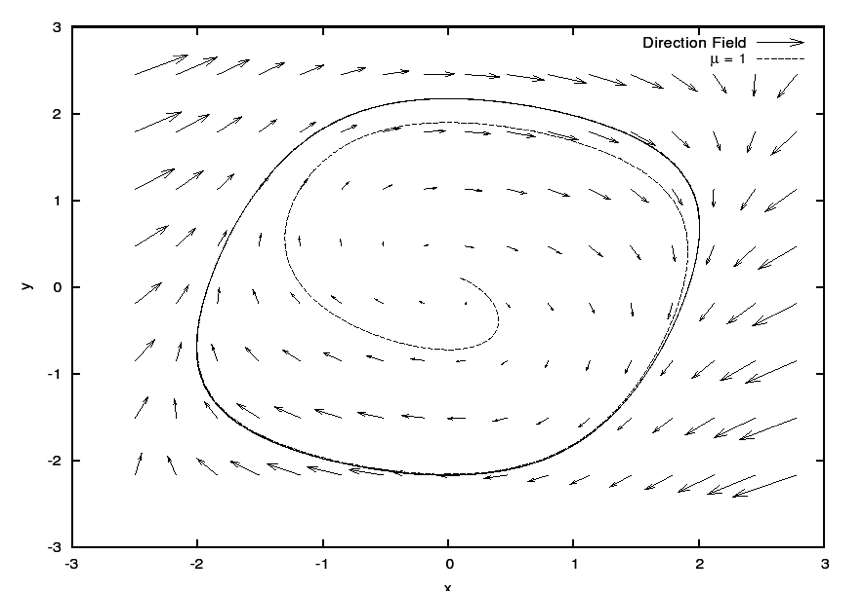
\includegraphics[scale=1]{dynamic_flow.png}
    \caption{连续时间动力学系统的相图}
    \label{fig:pha_spa}
\end{figure}
其中,我们称由所有维度的状态变量$\{x_1,x_2,\cdots,x_n\}$所张成的空间称为\textbf{相空间}。

对于一般的离散时间的动力学方程,我们可以用离散动力学方程\eqref{equ:map_dyna_sys}来描述:
\begin{equation}
    \begin{cases}
        \begin{aligned}
            x_1^{p+1} &= f_1(x_1^p,x_2^p,\cdots,x_n^p)\\
            x_2^{p+1} &= f_2(x_1^p,x_2^p,\cdots,x_n^p)\\
            \cdots &= \cdots \\
            x_n^{p+1} &= f_n(x_1^p,x_2^p,\cdots,x_n^p)
        \end{aligned}
    \end{cases}\label{equ:map_dyna_sys}
\end{equation}
其中$p\in \mathbb{N}$表示离散系统的迭代次数,即离散的时间指标。

\subsection{线性动力学系统}
在物理学中,我们比较熟悉的系统很多都是用线性方程描述动力学规律,即所谓的线性系统。线性方程很容易求解并且具有一些很简单的特性(如叠加原理)。在\eqref{equ:ode_dyna_sys}中,若$f_i(i=1,2,\cdots,n)$均为各自变量的线性函数,则我们的动力学系统即为一线性系统。连续时间线性系统可以用矩阵表示:
\begin{equation}
    \dot{x}=Ax
\end{equation}
其中$x$表示由所有状态变量构成的列向量,$A$为$n\times n$的矩阵($A_{ij}\in\mathbb{R}$)。

离散时间的线性动力学方程也可以用矩阵来表示:
\begin{equation}
    x_{n+1}=Ax_n
\end{equation}
其中$x$表示由所有状态变量构成的列向量,$A$为$n\times n$的矩阵($A_{ij}\in\mathbb{R}$),下标$n$表示系统的迭代次数,即离散的时间指标。

例如一个一维的连续时间线性系统$\dot{x}=3$,很容易求解其运动学方程为$x(t)=3t$,对应我们的一维匀速直线运动;再如系统$\dot{x}=-2x$,可以求解得到运动学方程为$x(t)=Ce^{-2t}$($C$为常数)。

\subsection{非线性动力学系统}
在实际中,许多物理现象乃至其他一些自然现象或者是社会现象毕竟是很复杂的,它们的动力学规律往往需要使用非线性方程表示。这些非线性方程除极少数外,一般都不存在解析解,但是它们却具有与线性方程解的不同的一些独特性质,所以非线性动力学需要一些其他的方法来研究其性质。若在\eqref{equ:ode_dyna_sys}中,若$f_i(i=1,2,\cdots,n)$有任意一个为自变量的非线性函数,则我们的动力学系统即为非线性系统。如一维弹性系统
\begin{equation}
    \ddot{x}+\omega^2x=0
\end{equation}
再如电子管振荡器中的范德波尔方程
\begin{equation}
    \ddot{x}+\alpha(x^2-1)\dot{x}+\omega^2x=0
\end{equation}

%由于在非线性系统中不易求得解析解,因此我们通常讨论非线性系统随时间的演化规律。在非线性系统中有一些特殊的性质,
我们将满足$\dot{x}=0$(连续时间系统)和$x_{n+1}=f(x_n)=x_n$(离散时间系统)的点$x^*$称为系统的\textbf{不动点}。在不动点处,系统状态变量不随时间发生变化。在连续时间系统中,我们将满足$T_{t^*}(x)=x$的轨道称为\textbf{周期轨道},周期为$t^*$,即粒子经过$t^*$时间后会回到起点;在离散时间系统中,我们将满足$x_{n+T}=x_n$的点称为\textbf{$T$周期点},周期为$T$,即粒子经过$T$次迭代又回到了起点。

\section{混沌系统}

混沌是非线性确定动力系统呈现出具有随机性的运动形态,即在一个确定性系统中,存在着貌似随机的不规则运动,其行为表现为不可重复、不可预测,这就是混沌现象。混沌是非线性动力系统的固有特性,是非线性系统普遍存在的现象。混沌具有确定性、初值敏感性、不可预测性。

当系统作一般的规则运动时,无法避涨落所引起的初始条件的微小变化一般只引起运动状态的微小差别,即初始状态接近的轨道始终是接近的,从而人们可以对系统的运动作出预测。然而混沌却不然,它具有对初始条件的敏感依赖性,即初始条件的微小差别常常使轨道按指数形式分开。洛伦兹也曾戏称混沌运动对初始条件的敏感依赖性为“蝴蝶效应”。

对于一个实际系统,由于无法避免内部涨落和外部环境噪声等因素的影响,初始状态的微小差别难以避免,因此混沌对初始状态的这种敏感依赖性必然会导致运动的不确定性与随机性。由于这种随机性,混沌系统在有限的相空间中必然要有折叠,否则轨线就只能是封闭曲线(规则的周期运动)或延伸到无穷远(发散解)。对于连续时间动力学系统,混沌只可能出现在三维及以上的自治系统(微分方程中不显含时间)中。

洛伦兹系统就是1963年E.Lorenz研究模拟大气在地表受阳光加热时的情形时得到的混沌系统:
\begin{equation}
    \begin{cases}
        \dot{x}=\sigma(y-x)\\
        \dot{y}=x(\rho-z)-y\\
        \dot{z}=xy-\beta z
    \end{cases}\
\end{equation}
其中$x$、$y$、$z$分别为与对流强弱、对流引起的水平温差和垂直方向温差有关的变量,$\sigma$、$\rho$和$\beta$分别与普兰多(Prandtl)数、瑞利(Rayleigh)数和容器大小有关的参数,在用计算机求上式的数值解时,洛伦兹发现,在参数取适当值时,解具有非周期性与随机性。随后Henon和R\H ossler等人也得到了类似的结果。

李雅普诺夫(Lyapunov)指数是表示相空间相邻轨迹的平均指数发散率的一个数值特征,是描述混沌现象的一个重要指标,对于一个映射$x_{n+1}=f(x_n,\alpha)$($\alpha$为参数),其李雅普诺夫指数的计算公式如下:
\begin{equation}
    \lambda(\alpha)=\lim_{n\to \infty}\dfrac{1}{n}\sum_{k=0}^{n-1}\ln{|\dfrac{df(x_k,\alpha)}{dx}|}
\end{equation}
其中$\alpha$表示动力学方程中的参数,$k$表示演化的离散时间指标。李雅普诺夫指数是用于识别混沌运动的重要特征。当$\lambda<0$时,映射系统收敛于某一不动点;当$\lambda=0$时,系统进行周期运动;当$\lambda>0$时,系统处于混沌状态。

关于混沌系统性质的讨论有很多,但是一般的方法直接观察系统的状态变量随时间的变化,即使观察时间很长,也不一定能看出规律。如果不对它作进一步的加工分析,很难了解其运动的性质和有关频谱成分等方面的信息,从而难以区分混沌和其他形式的震荡。当运动很复杂时,相空间中的轨迹可能是混乱一片甚至是充满某一区域而看不出什么规律。

为了研究复杂的非线性系统特别是混沌系统,通常有以下几种方法来进一步分析各种运动的特征。\textbf{频闪采样法}每隔一定时间观察轨迹上的代表点(采样点),这样,原来在相空间的连续运动就被一系列离散点$P_0$、$P_1$、
$P_2$、$\cdots$所代表,不同类型的运动可得到不同形态的采样结果,可以由此来分析其运动的性质。\textbf{庞加莱截面法}在多维相空间$\{x_1,x_2,\cdots,x_n\}$中选取一截面$f(x_i)=0$(此截面称为庞加莱截面),观察运动轨迹与此截面的截点(称为庞加莱点),则原来相空间的连续运动就被就被这些离散点$P_0$、$P_1$、
$P_2$、$\cdots$之间的映像所表示。\textbf{相空间重构法}选取一时间延迟量$T$,取$x(t)$、$x(t+T)$、$x(t+2T)$、$\cdots$、$x(t+mT)$为坐标画m维轨线,这样m个维度的变量随时间的变化隐含着整个系统的动力学规律,例如当相空间维度很高时,我们可以取$m=3$来重构高维的相空间,而三维的相空间我们则可以用图来形象化的描述。\textbf{功率谱法}是指任意函数都可以展开为一组基函数的线性组合,在物理中可理解为基频和一系列谐频的叠加,我们便可从频域分析原系统的动力学特征。



\section{Koopman算符}
Koopman算符由B.O.Koopman于1931年引入,它作用在某个函数上,描述了函数的演化。若将系统的特性数据演化视为函数的演化,我们即可以用Koopman算符分析系统的特征。现实中的许多系统,由于其动力学的复杂性而难以用较准确的动力学方程来近似描述,而只能得到通过实验或观测得到的系统特征数据。我们希望利用系统的特征数据,通过Koopman算符得到系统的动力学特征。

\subsection{Koopman算符的定义}
对于离散时间动力学系统,设对于相空间$\mathbf{P}$上的任意一点$x_p\in \mathbf{P}$,有$x_{p+1}=T(x_p)$。其中$p$为迭代次数,$T$描述了相空间的迭代规律。定义作用在相空间函数$f(x)$上的Koopman算符$U$, 使得:
\begin{equation}
    Uf(x)=f(T(x))
\end{equation}

对于连续时间动力学系统,设对于相空间$\mathbf{P}$上的任意一点$x_p\in \mathbf{P}$,有$x_t=T(x_0)$。其中下标$t$为时间,$T$描述了相空间随时间的演化规律。定义作用在相空间函数$f(x)$上的Koopman算符$U_t$,使得:
\begin{equation}
    U_tf(x)=f(T_t(x))
\end{equation} 

其中$f(x)$为定义在相空间上的任意可观测函数,如粒子的坐标、动量、浓度、概率密度等等。

给定$f(x)$,若令函数$\tilde{f}(x)=f(T(x))$,则Koopman算符可以描述函数的演化
\begin{equation}
    \begin{aligned}
        Uf(x)=f(T(x))=\tilde{f}(x)       &,&\text{(离散时间系统)}\\
        U_tf(x)=f(T_t(x))=\tilde{f}_t(x) &,&\text{(连续时间系统)}
    \end{aligned}
\end{equation}

例如,对于一个一维线性动力学方程
\begin{equation}
    \dot{x}=-2x
\end{equation}
其运动学方程$x(t)=x(0)e^{-2t}$,因此我们可以将其描述为
\begin{equation}
    T_t(x)=xe^{-2t}
\end{equation}
设我们有一在相空间的可观测函数
\begin{equation}
    f(x)=x^2
\end{equation}
若用Koopman算符作用在该函数上,我们可以得到
\begin{equation}
    U_tf(x)=f(T_t(x))=f(xe^{-2t})=x^2e^{-4t}=\tilde{f}(x)
\end{equation}
即Koopman算符作用在函数上,描述了函数的演化
\begin{equation}
    \begin{aligned}
        x^2 \stackrel{U_t}{\longrightarrow} x^2e^{-4t} \\
        f(x) \stackrel{U_t}{\longrightarrow} \tilde{f}(x)
    \end{aligned}
\end{equation}

Koopman算符$U$是无穷维的线性算符,即:
\begin{equation}
    U(\alpha f_1(x)+\beta f_2(x))=\alpha Ug_1(x)+\beta Ug_2(x)
\end{equation}
设有一个函数$f(x)$,我们将其分解到一组函数上$g_i(x)$($i=1,2,\cdots,n$)
\begin{equation}
    f(x)=\sum_{i=1}^n\alpha_ig_i(x)
\end{equation}
则Koopman算符可以描述为
\begin{equation}
    Uf(x)=U\sum_{i=1}^n\alpha_ig_i(x)=\sum_{i=1}^n\alpha_iUg_i(x)=\sum_{i=1}^n\alpha_ig_i(T(x))
\end{equation}
即一个复杂函数的演化规律可以描述为一组简单函数演化规律的线性叠加。

\subsection{Koopman算符的本征值与本征函数}
Koopman算符$U$是一个线性算符,可以对其进行谱分解。设有一复数$\lambda$和一复标量函数$\phi(x)$,使得
\begin{equation}
    U\phi(x)=\phi(T(x))=\lambda\phi(x)
\end{equation}
则称$\lambda$为Koopman算符的\textbf{本征值},$\phi(x)$为Koopman算符的\textbf{本征函数}。

Koopman算符的本征值和本征函数具有以下性质:

\textbf{性质1}:若$\phi_1(x)$,$\phi_2(x)$分别是Koopman算符U对应于$\lambda$的本征函数,则$\psi(x)=\alpha\phi_1(x)+\beta\phi_2(x)$也是U的本征函数,对应本征值为$\lambda$:
\begin{equation}
    U\psi(x)=\psi(T(x))=\alpha\phi_1(T(x))+\beta\phi_2(T(x))=\alpha\lambda\phi_1(x)+\beta
    \lambda\phi_2(x)=\lambda\psi(x)
\end{equation}

\textbf{性质2}:若$\phi_1(x)$,$\phi_2(x)$分别是Koopman算符$U$相应于本征值$\lambda_1$,$\lambda_2$的本征函数,则$\psi(x)=\phi_1(x)\phi_2(x)$也是$U$的本征函数,相应本征值为$\lambda_1\lambda_2$: 
\begin{equation}
U\psi(x)=\psi(T(x))=\phi_1(T(x))\phi_2(T(x))=\lambda_1\lambda_2\phi_1(x)\phi_2(x)=\lambda_1\lambda_2\psi(x)
\end{equation}

特别的,若$\phi(x)$是Koopman算符$U$相应于本征值$\lambda$的本征函数,则$\phi^n(x)$也是$U$的本征函数,相应的本征值为$\lambda^n$:
\begin{equation}
    U\phi^n(x)=(\phi(T(x)))^n=(\lambda\phi(x))^n=\lambda^n\phi^n(x)
\end{equation}

本征函数$\phi(x)$是一个在相空间上特殊的可观测函数,若将其在一组函数空间$\{g_1(x),g_2(x),\cdots,g_m(x)\}$中表示
\begin{equation}
    \phi(x)=\sum_{i=1}^m\alpha_ig_i(x)
\end{equation}
则Koopman算符描述本征函数$\phi(x)$的演化规律可以用一组基函数的演化规律来描述:
\begin{equation}
    \begin{aligned}
        U\phi(x)&=\sum_{i=1}^m\alpha_iUg_i(x)=\sum_{i=1}^m\alpha_ig_i(T(x))\\
        U\phi(x)&=\lambda\phi(x)=\sum_{i=1}^m\lambda\alpha_ig_i(x)
    \end{aligned}
\end{equation}

\subsection{Koopman算符的本征函数与相空间划分}

在动力学系统中,Koopman算符的本征值与本征函数有着特殊的含义。根据本征函数的定义,我们有
\begin{equation}
    \begin{aligned}
        \phi(x_p)=  &=U\phi(x_{p-1})=\lambda\phi(x_{p-1})\\
                    &=\lambda U\phi(x_{p-2})=\lambda^2\phi(x_{p-2})\\
                    &\cdots\\
                    &=\lambda^{n-1}U\phi(x_0)=\lambda^n\phi(x_0)
    \end{aligned}
\end{equation}
其中$p$为时间因子,我们可以看到,Koopman算符的本征函数值随着时间的演化呈$1/\lambda$倍变化,这反映了一种特殊的函数演化规律,而这个特殊的函数就是我们的Koopman算符的本征函数。相较于无规则的混沌演化,这种有规律的演化则更容易观察研究,而由于本征函数$\phi(x)$的特殊性,其必然反映了某种相空间的性质。因此,探究Koopman算符的本征函数的意义就变得尤为重要。

特别的,当$\lambda=1$时,则本征函数$\phi(x_p)=\phi(x_{p-1})=\cdots=\phi(x_{p-0})$($p\in \mathbb{Z}$为时间指标),此时本征函数不随时间发生变化,即$\phi(x)=C$($C$为常数),这与动力学系统中的守恒量相对应。例如在能量守恒定律中,就对应一个能量函数不随时间发生变化$E(x_1,\dot{x}_1,x_2,\dot{x}_2,\cdots,x_n,\dot{x}_n,t)=C$,亦可反推该函数是Koopman算符的本征函数。

当$|\lambda|=1$时(即$\lambda=e^{i\theta}$),则本征函数$|\phi(x_p)|=|\phi(x_{p-1})|=\cdots=|\phi(x_{p-0})|$($p\in \mathbb{Z}$为时间指标),此时本征函数的模不随时间发生变化(而相位在发生变化),这也对应了动力学系统中的一种守恒量。例如在匀速圆周运动中的速度矢量。

此外,在动力学系统中,周期轨道也反映了一种守恒量,Koopman算符的本征函数也与周期轨道有着密切的联系。

对于一个复杂的动力学系统,我们往往难以刻画其整体的动力学演化规律,因为许多系统的相空间在不同区域有着不同的性质。但若我们能够将动力学系统的相空间划分为多个区域,而每个区域的动力学系统有着相似的规律,我们便可以按区域描述相空间的演化规律。而相空间的划分又有着多种角度,我们可以从不同的角度对相空间进行划分,从而更具体的描述相空间的演化规律。

Koopman算符的本征值为我们提供了一个划分相空间的思路。对于Koopman算符谱中$|\lambda|=1$的本征值对应的本征函数,计算相空间中所有点的本征函数值,则本征函数值的模相同的点属于一个不变集。不变集中对应动力学系统的守恒量。若能通过这些不变集将相空间进行划分,我们便能实现对相空间运动模式的分块描述。因此我们可以求得Koopman算符的本征函数,并通过Koopman算符的本征函数实现对相空间的划分。通过多个本征函数从不同角度对相空间的划分,我们便可以更具体的刻画相空间的性质。


\subsection{Koopman谱分析与动力学模式}\label{section:Koop_dyna}

由于Koopman算符本征函数对相空间划分的重要性,我们将通过数值计算求得Koopman算符的本征函数。Koopman算符作用在函数上,描述了函数的演化规律。为了能够精确的描述一个本征函数,我们可以选取一组基函数$g_1(x),g_2(x),\cdots,g_m(x)$,$x\in \mathbb{R}$,其张成了一个函数空间,对于在该函数空间的任意函数$f(x)$,我们都可以表示为
\begin{equation}
    f(x)=\sum_{i=1}^m\alpha_ig_i(x)
\end{equation}
若我们能描述该函数空间内所有基函数的演化,则可以在该函数空间中求得我们的本征函数$\phi(x)$。
\begin{equation}
    Ug_i(x)=g_i(T(x))=\tilde{g}_i(x)
\end{equation}

为了得到Koopman算符的本征函数,我们需要构造演化前与演化后的数据,通常采用构造数据矩阵的方式,设某$p$时刻的数据为$\{x_{p_1},x_{p_2},\cdots,x_{p_n}\}$,$x_i\in \mathbb{R}^n$,当时刻为$p+1$时,数据演化为$\{x_{p_1+1},x_{p_2+1},\cdots,x_{p_n+1}\}$,$x_i\in \mathbb{R}^n$,在选取的基函数${g_i(x)}$,$i=1,2,\cdots,m$下,利用已知数据点将m个基函数及演化后的函数表示为在$\{x_{p_1},x_{p_2},\cdots,x_{p_n}\}$(称之为“演化格点”)下的列向量,从而构成两个$n\times m$的数据矩阵:
\begin{equation}
    \begin{aligned}
        K=(g_1(x_p),g_2(x_p),\cdots,g_m(x_p))=
        \begin{pmatrix}
        g_1(x_{p_1}) & g_2(x_{p_1}) & \cdots & g_m(x_{p_1}) \\
        g_1(x_{p_2}) & g_2(x_{p_2}) & \cdots & g_m(x_{p_2}) \\
        \vdots       & \vdots       & \ddots & \vdots \\
        g_1(x_{p_n}) & g_2(x_{p_n}) & \cdots & g_m(x_{p_n})
        \end{pmatrix}
    \end{aligned}
\end{equation}
\begin{equation}
    \begin{aligned}
    L=&(g_1(x_{p+1}),g_2(x_{p+1}),\cdots,g_m(x_{p+1}))\\
    =&(\tilde{g}_1(x),\tilde{g}_2(x),\cdots,\tilde{g}_m(x))=
        \begin{pmatrix}
        g_1(x_{p_1+1}) & g_2(x_{p_1+1}) & \cdots & g_m(x_{p_1+1}) \\
        g_1(x_{p_2+1}) & g_2(x_{p_2+1}) & \cdots & g_m(x_{p_2+1}) \\
        \vdots         & \vdots         & \ddots & \vdots \\
        g_1(x_{p_n+1}) & g_2(x_{p_n+1}) & \cdots & g_m(x_{p_n+1})
        \end{pmatrix}
    \end{aligned}
\end{equation}

其中$K$我们称为演化前矩阵,$L$称为演化后矩阵,$K$、$L$的每一列为相空间在一组点在某个基函数上的取值,当相空间的点数足够多时,可以视矩阵的每一列为一个基函数的离散数据表示,$K$、$L$则可以看作是多个基函数的组合,分别表示演化前的基函数和演化后的基函数,而演化后的基函数又可以看作一个新的函数,视为Koopman算符作用在基函数上得到。于是$K$、$L$之间的关系可由Koopman算符表示
\begin{equation}
    UK=L
\end{equation}
Koopman算符的矩阵表示可由上式确定,因此我们可以通过上式求得Koopman算符的矩阵表示,进一步求得Koopman算符的本征值与本征函数。

% 以Logistic映射为例,我们介绍Koopman分析的算法实现与具体步骤,不失一般性,我们取特定的参数$\gamma=4$,此时Logistic映射表现为混沌状态,此时Logistic映射的动力学方程可以描述为
% \begin{equation}
%     x_{n+1}=f(x_n)=4x_n(1-x_n),x_n\in [0,1],n=1,2,3,\cdots
% \end{equation}

% 该系统为一维系统,相空间范围为$[0,1]$,该系统存在两个不动点:$0$和$3/4$。我们首先根据该映射方程产生一组迭代数据,设我们产生的迭代数据的数量为$n+1$。则每个数据点可以表示为$x_i,i=1,2,\cdots,n+1$,为了得到“演化前数据”和“演化后数据”,我们将这组迭代产生的数据构造为$\{x_1,x_2,\cdots,x_n\}$与$\{x_2,x_3,\cdots,x_{n+1}\}$,并根据这两组数据构造出数据矩阵$K$与$L$。

在构造矩阵$K$与$L$时,我们需要选定一组基函数${g_i(x)},i=1,2,\cdots,m$,基函数的选取对我们计算本征函数的结果至关重要,于是我们将从多个角度讨论基函数的选取对本征函数的影响。基函数的选取至关重要,为了能较好的表示出Koopman算符的本征函数,需要一组较完备的基函数作为算符作用的可观测量,可以选取Gauss基函数、Fourier基函数、Legendre基函数。然而上述基函数只有在数量趋于无穷时才具有完备性,我们希望基函数的数量足够多,然而为了相空间的数据点能够较好的表示每个基函数,基函数的数量又不宜超过演化格点的数量,此外考虑到计算量的因素,我们只能将基函数的数量设为某个有限值。此外由于相空间粒子分布的不均匀性,我们还可以取不同分布的基函数。总之,基函数的选取有多重形式,而基函数的选取会影响到本征函数的计算,因此基函数的选取至关重要。

在选取合适的基函数与构造数据矩阵K与L后,我们即可以根据$UK=L$计算求得Koopman算符的矩阵表示以及本征值与本征函数,通常我们会得到n个本征值与本征函数,而在这些本征值中,我们比较关心的是本征值(或者本征值的模)接近1的本征函数,因为本征值为1的本征函数反映了相空间中一条随时间演化不变的轨道,这种轨道即是系统的一个关键特征,而由于我们的数值计算误差,因此我们将选取接近1的本征值对应的本征函数。

Koopman算符对相空间的划分可以通过混沌系统的已知特性来得到验证,如在Logistic映射中有两个不动点,而我们得到的本征函数图像恰好在不动点以及不动点的原像处得到了本征函数的极值点,说明了本征函数能够体现系统的动力学特征;此外,我们还可以通过验证动力学系统的周期点与周期轨道等特征,对比Koopman算符的本征函数,以此观察Koopman算符分析动力学系统的可行性。

Koopman算符理论上能够区分相空间的不同区域的性质,对于具有噪声的数据和涨落的演化规律,Koopman算符同样可以通过控制函数空间的精细度来对相空间进行粗细粒度的划分,因此Koopman算符具有鲁棒性:即使我们的演化有噪声的影响,如探究噪声中常见的高斯白噪声,我们同样可以对相空间进行粗粒度的划分。这在我们探究动力学系统中的演化规律中尤为重要。

\subsection{动力学系统的符号动力学与“边界点”}

符号动力学起源于动力系统的抽象拓扑理论的研究,并从20世纪60年代起逐渐在应用于一维映射的研究过程中得到发展和完善。符号动力学是研究符号动力系统的学科,这种系统的状态均可表示为有限个符号的无穷序列,而由任一状态点引出的运动轨道可由表示该状态的无穷序列通过简单的移位规则来确定。许多复杂动态系统均可经过变换等价于这类系统,从而可通过对比较简单的符号动力系统的分析来研究一般动力系统的行为。这种方法特别在混沌等复杂行为研究中占有重要地位。符号动力系统在其他领域也有广泛的应用。例如研究离散事件动态系统控制问题的代数方法就与符号动力学有密切的联系。

符号动力学是实际动力系统的抽象和概括。对于一个相空间的离散动力学系统,我们可以依据不同的符号将相空间的不同区域命名,如使用符号“0”和符号“1”来讲相空间划分为两个区域。通过相空间的演化,又可以继续用有限个符号来更加细致的划分相空间。理论上相空间中的每个点都可以用一个无穷的符号序列与之对应。当传统的微分理论难以对动力学系统分析时,我们可以使用粗粒度的符号动力学来研究动力学系统的性质。即使一般的数值方法行不通,符号动力学仍可以对系统进行定性分析。

Logistic映射就是一个可用符号动力学很好描述的典型,Logistic映射的动力学方程
\begin{equation}
    x_{n+1}=f(x_n)=\gamma x_n (1-x_n ),x_n∈[0,1],\ n=1,2,3,\cdots
\end{equation}
这里我们取$\gamma=4$,Logistic映射的迭代过程使它成为一个经典的混沌系统,符号动力系统也被视为混沌系统的原型,进而还可将符号动力系统的运动特征作为混沌的描述并成为混沌的一种严格的数学定义。Logistic映射的相图与符号动力学的划分可由下图表示:
\begin{figure}
	\centering
	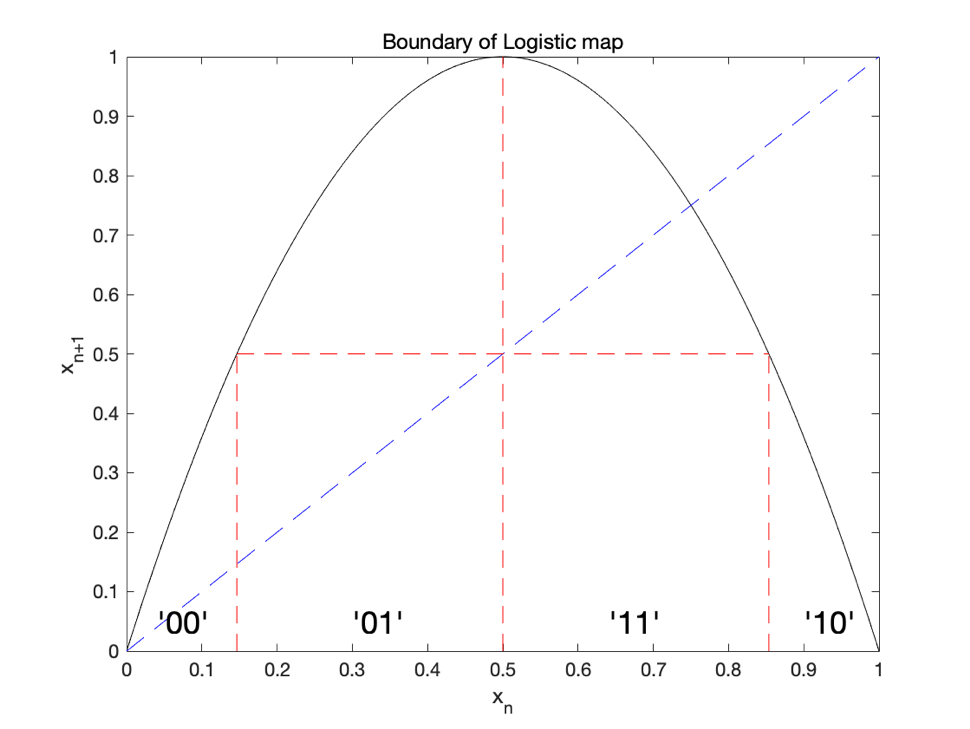
\includegraphics[scale=0.6]{logistic_symbolic.png}
    \caption{Logistic映射的符号动力学划分}
    \label{fig:logi_symb}
\end{figure}
Logistic映射的动力学过程可以看作是在一维相空间上的拉伸再折叠的过程,在折叠的临界点处$x=\frac{1}{2}$我们将其作为一个“临界点”,在临界点的两边我们分别标记区域为“0”和"1"。而在"0"区域的相空间$x\in [0,\frac{1}{2}]$中,其下一步演化的位置即存在演化为"0"的点,也存在演化为"1"的点。这样,我们可以根据该区域一次演化的结果进行更进一步的划分,则“0”区域的相空间又可以划分为"00"和"01"的相空间;同理,“1”区域的相空间可以划分为"11"和"10"的相空间。若将二次演化乃至多次演化作为划分符号动力学相空间的评判标准,则我们可以用符号动力学标记任意精度的相空间区域。特别的,在极限情况下,当我们演化的次数足够多时,我们可以对相空间的每个足够小的区域都划分出来,即相空间的每个点都对应一组无穷符号序列。

在符号动力学中,一个最关键的问题就是如何寻找“边界点”,\text{边界点}是指在符号动力学中可以划分相空间不同区域的临界点,如在Logistic映射中,$x=\frac{1}{2}$就是一个“边界点”,根据其演化我们还可以找到一次演化的边界点$x=\frac{1}{2}\pm\frac{\sqrt{2}}{4}$,以此类推。所以,若能找到系统的“边界点”,便可以通过符号动力学对其相空间进行划分。

Koopman算符的本征函数能够划分相空间区域的不同性质,而符号动力学的边界点也是反映了相空间区域的划分。当相空间的性质足够简单时,我们对其划分的标准就更单一。于是我们可以认为,此时Koopman算符的本征函数对相空间的划分恰好就是反映了符号动力学中的“边界点”对相空间的划分。我们将在后面的例子中继续探究这两者之间的对应关系。Koopman算符的本征函数恰能反映符号动力学的“边界点”,这也为我们寻找符号动力学的“边界点”提供了一个有效的方法。

\subsection{Koopman算符的函数空间}
% Rectangle Gauss Fourier Legendre
\subsubsection{正交完备基函数簇}
在\ref{section:Koop_dyna}节的讨论中,我们要选择一组基函数${g_i(x)},i=1,2,\cdots,m$来构造数据矩阵$K$与$L$,这里的基函数即限定了我们的函数空间,我们的本征函数由这组基函数来描述,因此,如何选择合适的基函数成为了一个至关重要的问题。

为了较好的表示出Koopman算符的本征函数,我们应选取一组正交完备的基函数来描述本征函数。完备性使得在此函数空间的任意函数都能且仅能得到一组唯一的线性组合。正交性使得基函数之间互不依赖。一般的,我们将定义在区间$[a,b]$上的一组基函数${g_i(x)}$的正交归一性用以下函数的内积来表示:
\begin{equation}
    <g_i,g_j>=\int_a^b{g_i(x)g_j(x)}dx=\delta_{ij}=
    \begin{cases}
        1,\ (i=j)\\
        0,\ (i\neq j)
    \end{cases}
\end{equation}

举一些基函数的例子。对于一维系统,设相空间为$x\in [0,1]$,我们在这个相空间范围内选取一组基函数${g_i(x)},i=1,2,\cdots,m$。考虑到正交性,对于最简单的一个例子就是矩形窗基函数:
\begin{equation}
    g_i(x)=
    \begin{cases}
        \sqrt{m},\ &(\dfrac{i-1}{m}\leqslant x<\dfrac{i}{m})\\
        0,\ &(x为其他)
    \end{cases},\ i=1,2,\cdots,m
\end{equation}
矩形窗基函数是一个局域化的函数,其结构足够简单,其所描述的函数空间总是能按照本征函数值区分相空间。

矩形窗基函数的每个函数之间没有任何冗余信息,这样很多函数都没有起到描述相空间的作用,为此我们可以将函数取为一组近似局域化的高斯基函数:
\begin{equation}
    g_i(x)=Cexp\left(-\dfrac{(x-x_i)^2}{2d_j^2}\right), \ x_i=\frac{i}{m}-\frac{1}{2m},\ i=1,2,\cdots,m
\end{equation}
其中C为高斯函数的归一化常数$C=\frac{1}{\sqrt{\sqrt{\pi}\sigma}}$。高斯基函数满足近似正交性,是一组近似局域性的全局基函数,每个函数都定义在整个相空间上,其形状类似一“波包”。其中有两个参数:波包中心$x_i$和波包宽度$d_j$。波包中心$x_i$表示高斯波包的中心位置,其选取通常应遍布大部分相空间,为了减少边界效应,一般情况下我们选取$x_i=\frac{i}{m}-\frac{1}{2m}$;波包宽度$d_j$描述高斯波包衰减到$\sqrt{\frac{1}{e}}$的距离,其选取应综合考虑相空间粒子的一步演化距离和函数之间的重叠,一般情况下我们选取$d_j=\frac{1}{2m}$。计算表明,使用高斯基函数可以得到较为清晰的动力学系统的相空间划分。

除了上述两个局域化的基函数,我们还可以考虑非局域化的基函数。如定义在$x\in [0,1]$上的傅里叶基函数
\begin{equation}
    g_k(x)=e^{ik(2\pi)x},\ k=-m,-(m-1),\cdots,m-1,m
\end{equation}
傅里叶基函数描述了每个频率的重要程度。再如多项式基函数
\begin{equation}
    g_i(x)=x^i,\ i=0,1,\cdots,m
\end{equation}
和其处于同一函数空间的定义在$x\in [-1,1]$上的勒让德基函数
\begin{equation}
    g_i(x)=\sqrt{\dfrac{2k+1}{2}}P_i(x),\ k=0,1,\cdots,m
\end{equation}

下图绘制了一维矩形窗基函数、高斯基函数、傅里叶基函数和勒让德基函数的图像
\begin{figure}
	\centering
	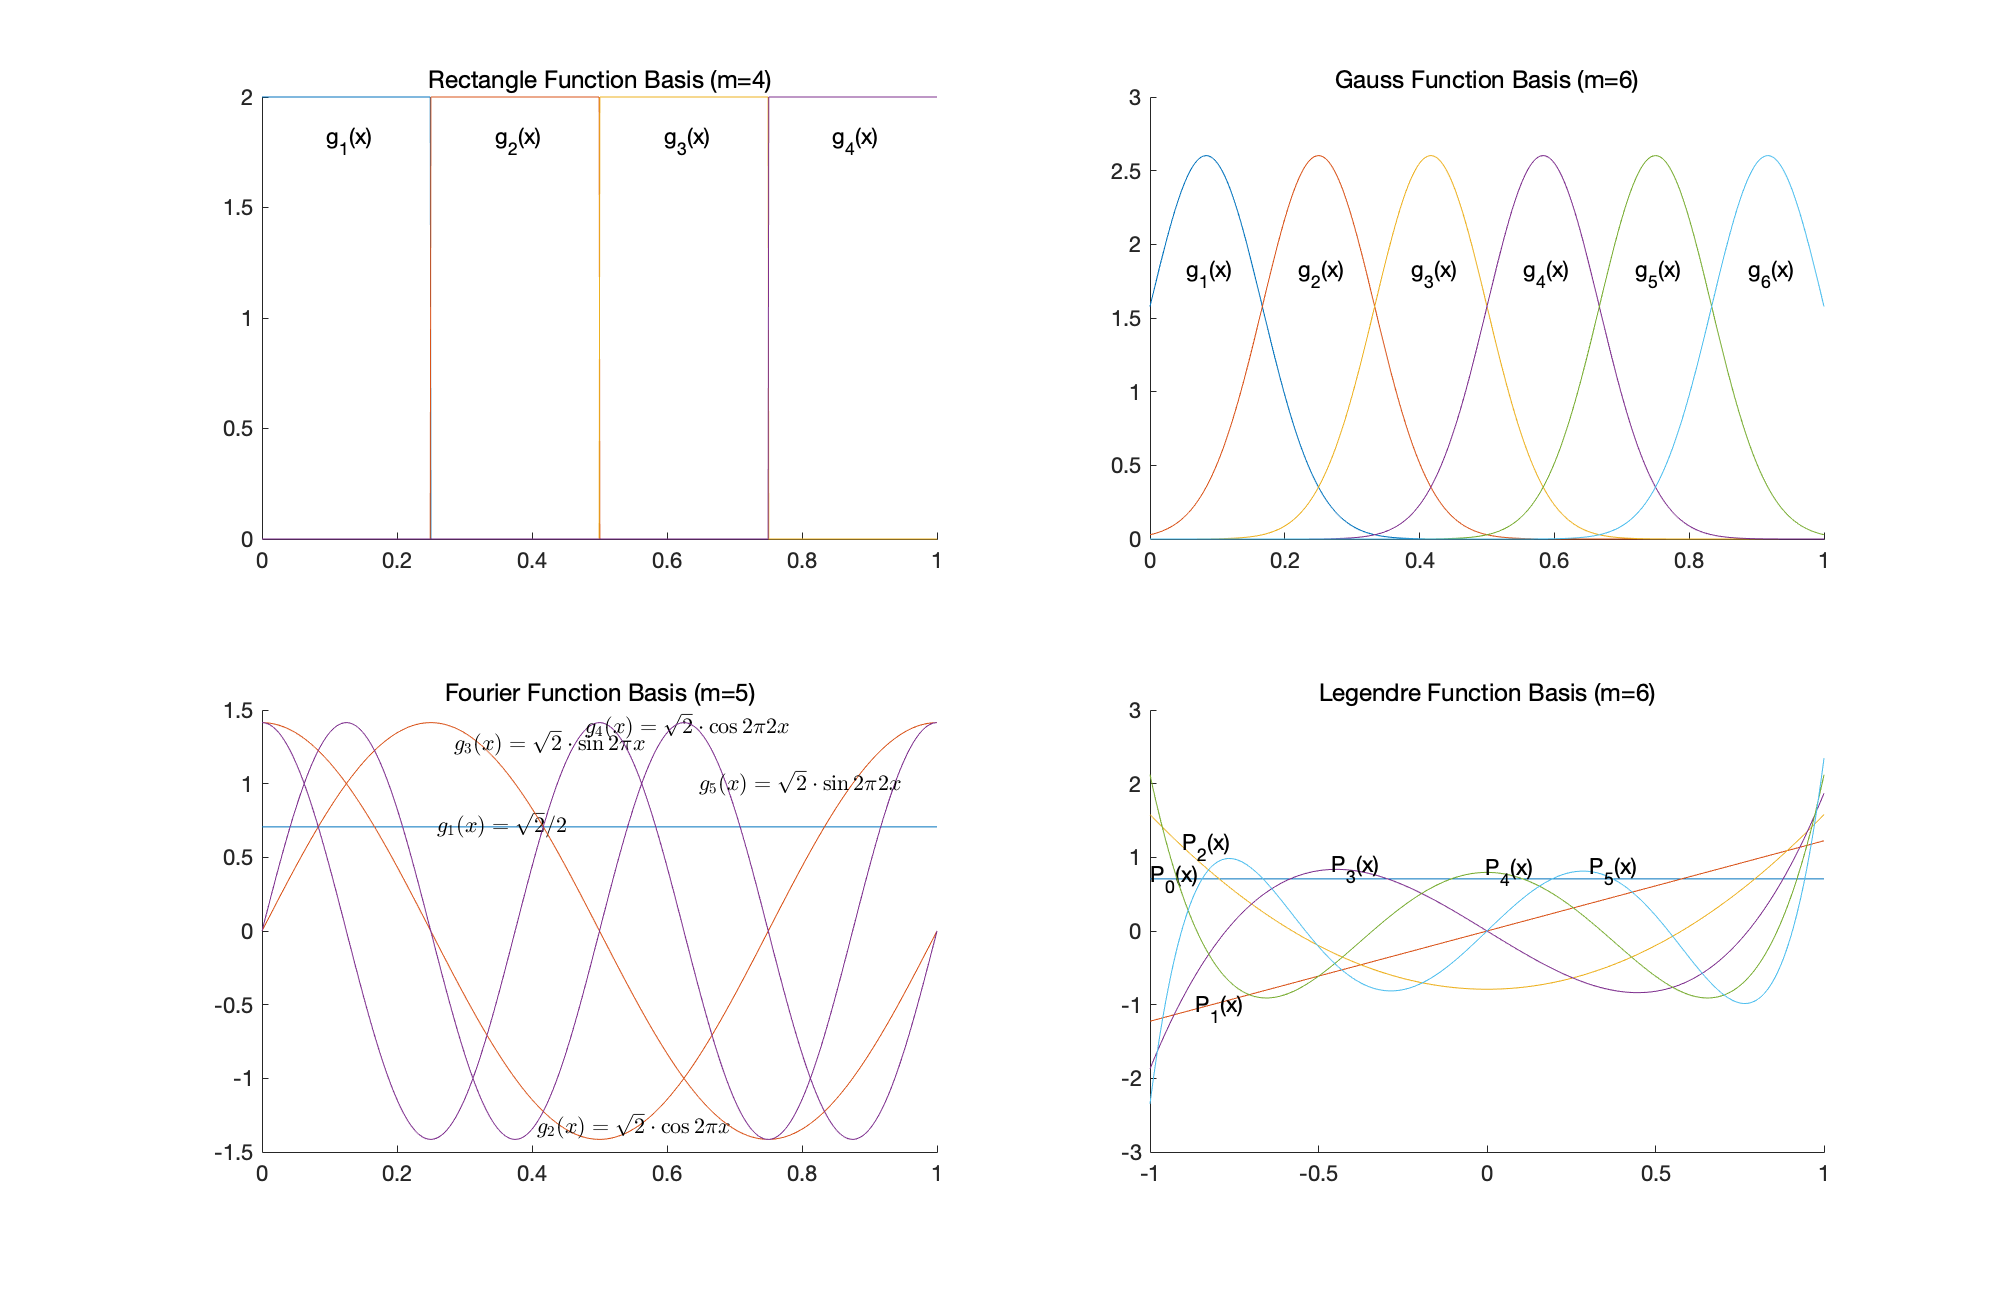
\includegraphics[scale=0.2]{function_basis}
    \caption{矩形窗、高斯、傅里叶、勒让德基函数图像}
    \label{fig:func_bas}
\end{figure}

对于高维系统,亦可以将上述方程扩展,如高维傅里叶基函数与高维高斯基函数。对于任意$n$位动力学系统,我们总是可以构造一组$n$维函数空间,将本征函数在此$n$维函数空间描述,我们便可以更准确的描述本征函数,从而对我们的相空间进行划分。

\subsubsection{自然演化的函数空间}

在\ref{section:Koop_dyna}节中,我们在动力学系统中可以选取一组合适的基函数,并将本征函数在此基函数中进行描述。这里考虑另一种取基函数的方法:自然演化的函数空间。对于在相空间$\mathbb{p}$中的系统状态变量$x_i$,我们取一个初始状态$x_i$,并将其进行$n$次演化,得到一组随时间演化的状态变量$(x_i,x_{i+1},\cdots,x_{n+i-1})^T$,这组状态变量也可以看做是相空间的一个$n$维函数,只不过其是由自然演化得到的。对于这样的一个基函数$g_i(x)=(x_i,x_{i+1},\cdots,x_{n+i-1})^T$,我们将Koopman算符作用在$g_1(x)$上可以得到
\begin{equation}
    Ug_i(x)=U(x_i,x_{i+1},\cdots,x_{n+i-1})^T=(x_{i+1},x_{i+2},\cdots,x_{n+i})^T=g_{i+1}(x)
\end{equation}

我们连续的取$m$个这样的自然演化的基函数$g_i(x)=(x_i,x_{i+1},\cdots,x_{n+i-1})^T$,并利用自然演化的基函数构造数据矩阵$K$和$L$:
\begin{equation}
    K=\{g_1(x),g_2(x),\cdots,g_m(x)\}=
    \begin{pmatrix}
        x_1 & x_2 & \cdots & x_m \\
        x_2 & x_3 & \cdots & x_{m+1} \\
        \vdots         & \vdots         & \ddots & \vdots \\
        x_n & x_{n+1} & \cdots & x_{n+m-1}
    \end{pmatrix}
\end{equation}
\begin{equation}
    L=\{g_2(x),g_3(x),\cdots,g_{m+1}(x)\}=
    \begin{pmatrix}
        x_2 & x_3 & \cdots & x_{m+1} \\
        x_3 & x_4 & \cdots & x_{m+2} \\
        \vdots         & \vdots         & \ddots & \vdots \\
        x_{n+1} & x_{n+2} & \cdots & x_{n+m}
    \end{pmatrix}
\end{equation}
$K$、$L$的每一列为相空间在一个初始点上的演化,当演化次数$n$足够多时,我们可以用这组演化来表示一个描述相空间的自然函数,$K$、$L$可以看作是多个基函数的组合,分别表示演化前和演化后的自然函数。同样的,数据矩阵$K$、$L$之间的关系可由Koopman算符表示
\begin{equation}
    UK=L
\end{equation}

不同于\ref{section:Koop_dyna}节中我们构造的函数空间,自然演化的函数空间仅由系统的动力学演化得到,其更能反映动力学系统的本征行为。我们可进一步求出在自然演化的基函数中Koopman算符的本征函数并以此来划分相空间。



%% 本章参考文献
% \ifx\usechapbib\empty
% \nocite{BSTcontrol}
% \setcounter{NAT@ctr}{0}
% \bibliographystyle{buptgraduatethesis}
% \bibliography{references}
% \fi

\chapter{典型混沌系统的Koopman分析}

\section{Tent映射}
\begin{equation}
    x_{n+1}=f(x_n)=1-2|x-\frac{1}{2}| ,\ x_n\in [0,1], n=1,2,3,\cdots
\end{equation}

\section{Logistic映射}
Logistic映射来源于生态学中的虫口模型,其动力学方程可描述为
\begin{equation}
    x_{n+1}=f(x_n)=\gamma x_n(1-x_n),\ x_n\in [0,1], n=1,2,3,\cdots
\end{equation}

通过非线性动力学的知识可以得到,该系统在$\gamma$取不同值时表现出不同的动力学行为。当$0<\gamma<1$时,系统最终都会渐进的趋于0;当$1<\gamma<3$时,系统会收敛到一个不动点,该不动点的值为$x^*=(\gamma-1)/\gamma$,此时系统的极限行为会趋于该不动点的值;当$3<\gamma<3.57$时,系统的迭代会出现周期行为,随着r的增大,周期的长度也会相应的增加,例如2周期,4周期,8周期等;当$3.57<\gamma<4$时,系统的迭代会在周期类型和混沌类型之间来回切换;直到$\gamma=4$时,系统处于完全混沌的状态。在我们的Koopman分析中,我们取$\gamma=4$的一个特例,通过Logistic映射的动力学方程演化出一系列的数据,作为Koopman分析的源数据,以此来分析Logistic映射的系统特征。

\section{Henon映射}
Henon映射是由法国数学家Michel H\'{e}non提出的,以此作为Lorenz模型的Poincar\'{e}界面的简化模型。Henon映射是一个可以产生混沌现象的离散时间动态系统,其迭代方程可以描述为

\begin{equation}
    \begin{cases}
        x_{n+1}=y_n+1-ax_n^2\\
        y_{n+1}=bx_n
    \end{cases}\ x,y\in [-1.5,1.5]
\end{equation}

在经典的Henon映射中,我们通常取$a=1.4$与$b=0.3$,此时系统表现出混沌现象。在我们的Koopman分析中,我们在取上述参数值的情况下,通过Henon映射的迭代方程演化出一系列的数据,作为Koopman分析的源数据,以此来分析Henon映射的系统特征。


\section{Lorenz系统}
Lorenz系统是1963年由Edward Lorenz提出的描述空气流体运动的一个数学模型,通常用Lorenz方程来描述
\begin{equation}
    \begin{cases}
        \dot{x}=\sigma(y-x)\\
        \dot{y}=x(\rho-z)-y\\
        \dot{z}=xy-\beta z
    \end{cases}\
\end{equation}

该方程描述了一个三维相空间的三个分量对时间的变化率,是一个连续时间动态系统。Lorenz系统具有非线性、非周期性和确定性的性质。参数$\sigma$,$\rho$,$\beta$取不同值时Lorenz系统表现出不同的动力学行为。如在$\rho<1$时,系统只有一个不动点,即原点,所有轨道的长期行为都趋于原点;当$\rho=1$时系统发生了叉式分叉,在$\rho>1$时出现了两个不动点,不动点的稳定性可由其他参数满足的条件确定;当我们将三个参数取一组特定的值$\rho=28$,$\sigma=10$,$\beta=8/3$时,Lorenz方程的解是混沌的,相空间会存在两个奇异吸引子。Lorenz系统的这种动力学特征用传统的非线性动力学知识是比较难分析的,我们将在取上述参数的条件下,通过Lorenz微分方程演化出相空间的一条轨道,作为Koopman分析的源数据,以此来分析Lorenz系统的特征。

%% 本章参考文献
% \ifx\usechapbib\empty
% \nocite{BSTcontrol}
% \setcounter{NAT@ctr}{0}
% \bibliographystyle{buptgraduatethesis}
% \bibliography{references}
% \fi

% \chapter{功能测试}

%% 本章参考文献
% \ifx\usechapbib\empty
% \nocite{BSTcontrol}
% \setcounter{NAT@ctr}{0}
% \bibliographystyle{buptgraduatethesis}
% \bibliography{references}
% \fi

\chapter{总结与展望}
\section{问题及整改方案}
1.如何精确的用一些随机梯度下降算法求得精简的本征值。以及如何跳出局部最优解。
2.随着基函数的增多,本征函数的划分也变得更精确,如何通过粗粒度的划分来实现细粒度的划分。
3.如果原方程加了噪声,会对Koopman算符本征函数有何影响。
4.Koopman算符的本征函数是否具有鲁棒性。
5.如何确定边界点的层次。
6.能否用通用的方法画出动力学系统的分界线。
7.本征函数的最大值最小值分别表示什么含义。
8.基函数的变化是如何影响本征函数的。
以上都是在课题中遇到的问题,今后会继续加强对这些问题的思考与完善,并将这些思考过程择重点记录到论文中。
\section{本研究课题可能的创新之处}
\begin{description}
    \item[给出了一个分析动力学系统的普适性方法]

    线性的动力学系统通过经典的动力学理论已经能够得到较好的解析分析方法,而非线性动力学系统的分析方法也有诸多理论用于系统的分析,比如通过不动点的线性化分析得到不动点近邻区域的系统演化特征。而对于复杂的非线性动力学系统比如混沌系统,传统的非线性动力学分析方法有其局限性。目前有许多分析非线性系统的行为的定性技巧,但是这些技巧没有一个对所有非线性系统都适用,大多数的技巧都只适用与一些特殊的情形。而我们提出的Koopman分析方法的理论和算法适用所有的动力学系统,因此在很多系统上都具有极其广泛的应用前景。

    \item[从函数演化的角度分析常见的混沌系统并验证Koopman分析的有效性]
     
    对于常见的一些混沌系统,其动力学特征已被很多前人研究过,我们使用Koopman分析方法分析其动力学特征去验证我们分析方法的正确性,同时给出了一种新的分析动力学系统的Koopman分析方法,即通过函数演化的角度去分析动力学特征。

    \item[给出了对于一般复杂系统的分析方法]
     
    通过Koopman分析在常见混沌系统中的特征提取,我们给出了对于一般复杂系统的分析方式,即使我们不知道系统的工作内部机制以及动力学方程,只需要得到系统的状态演化过程,便能对复杂系统进行定性的分析。由于其普适性,我们可以将Koopman分析应用到各种复杂问题上,如生物大分子的运动、流体系统、模式识别以及气候变化等。
 
\end{description}
%% 本章参考文献
% \ifx\usechapbib\empty
% \nocite{BSTcontrol}
% \setcounter{NAT@ctr}{0}
% \bibliographystyle{buptgraduatethesis}
% \bibliography{references}
% \fi

\chapter{开题报告}

\section{立项依据}
\subsection{研究目的与意义}
当今时代是一个信息时代,社会的发展充斥着各种信息交换,包括机械、能源、交通、化工、生物、航空航天等各项领域,然而在信息传递中愈发庞大的信息量中,如何有效的提取关键的信息是一个亟待解决的问题。

信息的具体表现形式是数据,数据和信息直接是相互联系的,数据是反映客观事物属性的记录。数据经过加工处理之后,就成为信息,而信息需要经过数字化转变成数据才能存储和传输。因此,数据分析也成为当下的一个热点问题。

随着数学与计算机等领域的发展,测量技术和计算能力的巨大改进,数据分析已成为一门新兴的学科应用在各个领域,并将继续发展。然而数据分析的方法多种多样,不同的数据分析方法的有效性也不同,很多数据的分析方法都依赖于数据的数学特征。我们寄希望于找到一个普遍的数据分析方法,通过研究数据从而了解其内部的抽象结构。

在许多实际系统中,我们通常可以得到一系列关于该系统的丰富数据,然而由于不了解其动力学原理或者系统过于复杂等原因无法用比较准确的动力学方程来近似描述。为了了解和研究这些系统,通常进行大量的实验或观测得到系统的特性数据。我们希望能够找到一种方法,仅通过系统数据的演化过程得到系统的一些演化特征,并在这些演化特征中提取出关键特征。如果我们能提取出复杂系统的关键特征,就能通过分析实际复杂系统的长期行为,并对系统的行为作出一定程度的预测。在我们的现实生活中,若将各种事件抽象为一种数据,并能提取出关键特征并进行预测,将具有很大的现实意义。

Koopman算符给我们提供了一个有效的数学工具。Koopman算法由B.O.Koopman与1931年引入,它作用在某个函数上,描述了函数的演化。若将系统的特性数据演化视为函数的演化,我们即可以用Koopman算符分析系统的特征。我们将用Koopman分析方法分析数据并作出一定程度的预测。

\subsection{国内外的研究现状}
关于数据分析与数据预测的方法有诸多理论。在本研究课题中采取Koopman算符进行数据的分析与预测。Koopman 算符由B. O. Koopman 于1931 年提出,能够描述系统可观察量随时间的演化,并可用来研究动力系统的各态历经性质,随后被证明与Liouville算符有着紧密联系。其早期的相关工作主要集中于统计力学系统和非线性动力系统中Koopman算符谱性质的解析研究。Mezić 曾在2004 年的一篇文章中探讨了利用Koopman算符的某些本征函数对确定性以及随机非线性动力系统进行各态历经划分的理论和方法,然后于2005 年发表的文章中再次对Koopman 算符进行了谱分析的理论研究,并根据结论提出了可以利用其谱特征对高维动力系统(如流体系统和生物分子系统)进行模型简化的可能性。,2009 年Rowley、Mezić 等发表了第一篇有关Koopman 算符谱分析应用于流体力学中的文章,文章中介绍了基于Arnoldi 算法的Koopman 谱分析和模式分解方法:利用流体系统速度场的测量数据,构建Koopman 算符的矩阵表示,然后通过特征分解得到一系列本征值及对应的本征模式(Koopman 模式)。其中,每一个Koopman 模式都描述了非线性系统的一种动力学特征,相应本征值则描述了该模式的变化规律。Budisic等人在2012 年总结了Koopman 谱分析的理论和应用:在给定系统数据中,可以求得Koopman 算符的三种特性量,分别为本征值、本征函数和Koopman 模式。其中本征函数可以用于对系统进行各态历经的划分,Koopman 模式则用来简化模型以及研究不同变量之间的相关性。Steven等人在2017年提出了另一种Koopman分析的观点(HAVOK)并用SVD及时间延迟嵌入定理对常见的混沌系统做出分析,并预测了波峰出现的时机。

\subsection{参考文献}
[1] 贾继莹. Koopman算符在一些动力系统中的算法和应用研究[D]. 2015.
[2] Brunton S L, Brunton B W, Proctor J L, et al. Chaos as an intermittently forced linear system[J]. Nature Communications, 2017, 8(1):19.
[3] Strogatz S H. From Kuramoto to Crawford: exploring the onset of synchronization in populations of coupled oscillators[J]. Physica D, 2000, 143(1-4):1-20.
[4] Hobson D. An Efficient Method for Computing Invariant Manifolds of Planar Maps[J]. Journal of Computational Physics, 1993, 104(1):14-22.
[5] Carles Simó. On the Hénon-Pomeau attractor[J]. Journal of Statistical Physics, 1979, 21(4):465-494.
[6] Pomeau Y, Berre M L. Dynamics of self-gravitating systems : Variations on a theme by Michel Henon[J]. Physics, 2014.
[7] Gaspard, P. Nicolis, G. Provata, A. Tasaki, S. Spectral signature of the pitchfork bifurcation: Liouville equation. Physical Review E, 1995.
[8] Gaspard P, Tasaki S. Liouvillian dynamics of the Hopf bifurcation[J]. Physical Review E, 2001, 64(5):056232.
[9] Korda M, Putinar M, Mezić, Igor. Data-driven spectral analysis of the Koopman operator[J]. 2017.
[10] Lan Y, Cvitanović P. Variational method for finding periodic orbits in a general flow[J]. Physical Review E, 2004, 69(1):016217.
[11] Steven H. Strogatz. Nonlinear dynamics and chaos: with applications to physics, biology, chemistry, and engineering [M]. Perseus Books Publishing, 2000
[12] Igor Mezić. Spectral Koopman operator in dynamical systems. Springer, 2017

\section{研究内容和目标}
\subsection{研究内容}
我们希望能够找到一种方法,仅通过系统数据的演化过程得到系统的一些演化特征,并在这些演化特征中提取出关键特征。Koopman算符给我们提供了一个有效的数学工具。Koopman算法由B.O.Koopman与1931年引入,它作用在某个函数上,描述了函数的演化。若将系统的特性数据演化视为函数的演化,我们即可以用Koopman算符分析系统的特征。

Koopman分析方法仅由系统的特性数据得到,理论上在数据足够多的情况下,我们可以得到系统的一切特征,如何提取出关键的系统特征(或者说是我们想要的系统特征)也是一个很复杂的问题;另一方面,我们在实际应用中的数据总是有限的,也会存在一定的误差,于是复杂系统的Koopman分析依赖于大量的系统数据支持。为了简化计算复杂度,而又不失Koopman分析的核心思想,我们可以先选取某些已知的动力学系统作为Koopman分析的对象。

线性的动力学系统通过经典的动力学理论已经能够得到较好的解析分析方法,而非线性动力学系统的分析方法也有诸多理论用于系统的分析,比如通过不动点的线性化分析得到不动点近邻区域的系统演化特征。而对于复杂的非线性动力学系统比如混沌系统,传统的非线性动力学分析方法有其局限性。我们试图将Koopman分析应用在某些混沌系统上,提取出混沌系统的系统特征,如果能抓住混沌系统的主要特征并进行定量的分析,就可以分析出混沌系统的长期行为,从而对混沌系统做一定程度上的预测。

混沌系统按照系统方程可以分为混沌映射(离散混沌系统)与混沌流(连续混沌系统),其本质是相同的。但由于在分析过程中需要用到数值计算,而数值计算对混沌映射与混沌流的影响是不同的:混沌映射的数值计算误差来源主要依赖于计算机的精度误差;混沌流的数值计算误差来源除了计算机的精度误差,其主要误差来源于系统时间间隔的选取。另一方面,混沌流的数值计算过程也可以转变为一个关于系统时间间隔的映射系统。因此,我们的Koopman分析方法以混沌映射系统为基础,分别讨论混沌映射系统与混沌流系统。

混沌系统按照系统维度可以分为一维、二维、三维与高维系统,不同维度的混沌系统在计算方法与计算复杂度上有一定区别。有一些常见的混沌系统,比如Logistic映射(一维映射),Henon映射(二维映射),Standard映射(二维映射),Lorenz系统(三维流),我们将选取几个典型的混沌系统作为分析对象,以验证Koopman分析的有效性。

% Koopman算符
% 考虑在相空间P上演化的离散动力系统:对于x_p∈P,x_(p+1)=T(x_p) 
% 定义作用在相空间函数g(x)上的Koopman 算符U, 使得:
% Ug(x)=g(T(x))
% Koopman算符描述了可观测量g的值沿相空间轨道的演化,若可观测量g在初始时刻的值g(x_0)为,则演化p步后可观测量g的值变为g(x_p )=U^p g(x_0)。
% 给定g(x),若令函数g ̃(x)=g(T(x)),则Koopman算符的作用为
% Ug(x)=g ̃(x)
% 因此Koopman算符的作用既可以看作映射T下g(x)函数值的演化,也可以看作函数形式的演化(g(x)→g ̃(x))。
% Koopman算符U是线性算符,即使动力系统本身是非线性系统。即:
%                 U(αg_1 (x)+βg_2 (x))=αUg_1 (x)+βUg_2 (x)
% 其中g_1 (x),g_2 (x)为相空间P上的任意标量函数,α,βϵC为任意标量。U是无穷维的算符,因此通过分析无穷维的线性算符U,能够体现有限维非线性系统的动力学特征。
% 许多实际的系统中,我们通常关注具有某些特征或意义的可观测量,这些量是定义在相空间的函数,由于其随时间变化的特征,它们通常是相应系统中Koopman算符的本征函数。Koopman曾用Koopman算符的谱性质研究动力系统的遍历性质。
% Koopman算符U是一个线性算符,可以对其进行谱分解,设一个复标量函数φ_k (x)为Koopman算符的本征函数,其相应的本征值为λ_k,则有
% Uφ_k (x)=φ_k (T(x))=λ_k φ_k (x),k=1,2,⋯
% 若φ_(k_1 ) (x),φ_(k_2 ) (x)分别是Koopman算符U相应于本征值λ_(k_1 ),λ_(k_2 )的本征函数,则ψ(x)=φ_(k_1 ) (x) φ_(k_2 ) (x)也是U的本征函数,相应本征值为λ_(k_1 ) λ_(k_2 ): 
% Uψ(x)=ψ(T(x))=φ_(k_1 ) (T(x)) φ_(k_2 ) (T(x))=λ_(k_1 ) λ_(k_2 ) φ_(k_1 ) (x) φ_(k_2 ) (x)=λ_(k_1 ) λ_(k_2 ) ψ(x)
% 特别的,若λ_k是U的本征值,相应本征函数为φ_k (x),则λ_k的n次方〖λ_k〗^n(n为整数)也是U的本征值,相应本征函数为〖φ_k〗^n (x)=(〖φ_k (x))〗^n:
%       U〖φ_k〗^n (x)=(〖φ_k (T(x)))〗^n=(〖λ_k φ_k (x)〗^n )=〖λ_k〗^n 〖φ_k〗^n (x),nϵZ,k=1,2,⋯
% 两类特殊的本征值和本征函数:
% 1.当本征值为λ_k=1时,设相应本征函数为φ_k (x),则φ_k (x_p )=Uφ_k (x_(p-1) )=φ_k (x_(p-1) )=⋯=φ_k (x_0 ) (pϵZ为时间指标),即沿着一条轨道本征函数值不随时间变化,这与物理系统中的守恒量相对应。
% 2.当本征值为λ_k=e^iθ(θ为实数)时,设相应的本征函数为φ_k (x),则φ_k (x_p )=Uφ_k (x_(p-1) )=e^iθ φ_k (x_(p-1) )=⋯=e^ipθ φ_k (x_0 ),即沿着一条轨道本征函数值模不变,而相位在变化。
% Koopman算符的谱中模为1的本征值|λ_k |=1对应的本征函数的性质为在动力系统相空间寻找不变集和周期结构提供了一种标准:计算相空间中给定所有点在这些本征函数上的值,则本征函数值(或本征函数值的模)相同的点属于相空间的一个不变集(但并不一定是最小不变集)。
% 为了得到Koopman算符的本征函数,我们通常采用构造数据矩阵的方式,设某p时刻的数据为{x_(p_1 ),x_(p_2,),⋯x_(p_n ) } ,x_i∈R^N,当时刻为p+1时,数据演化为{x_(p_1+1),x_(p_2+1,),⋯x_(p_n+1) } ,x_i∈R^N,我们可以选取一组基函数{g_j (x)},j=1,2,⋯m后,利用已知数据点将m个基函数及演化后的函数表示为在{x_(p_1 ),x_(p_2,)⋯x_(p_n ) }(称之为“演化格点”)下的列向量,从而构成两个数据矩阵:
% K=(g_1 (x),g_2 (x),⋯g_m (x))=(■(g_1 (x_(p_1 ) )&g_2 (x_(p_1 ) )  ⋯&g_m (x_(p_1 ))@⋮&⋱&⋮@g_1 (x_(p_n ) )&g_2 (x_(p_n ))⋯&g_m (x_(p_n ))))
% L=(g ̃_1 (x),g ̃_2 (x),⋯g ̃_m (x))= (■(g_1 (x_(p_1+1) )&g_2 (x_(p_1+1) )  ⋯&g_m (x_(p_1+1))@⋮&⋱&⋮@g_1 (x_(p_n+1) )&g_2 (x_(p_n+1))⋯&g_m (x_(p_n+1))))
% 其中K我们称为演化前矩阵,L称为演化后矩阵,K、L的每一列为相空间在一组点在某个基函数上的取值,当相空间的点数足够多时,可以视矩阵的每一列为一个基函数的离散数据表示,K、L则可以看作是多个基函数的组合,分别表示演化前的基函数和演化后的基函数,而演化后的基函数又可以看作一个新的函数,视为Koopman算符作用在基函数上得到。于是K、L之间的关系可由Koopman算符表示
% UK = L
% Koopman算符的矩阵表示可由上式确定,因此我们可以通过上式求得Koopman算符的矩阵表示,进一步求得Koopman算符的本征值与本征函数。

% 常见的混沌系统 
% Logistic映射来源于生态学中的虫口模型,其动力学方程可描述为
% x_(n+1)=f(x_n )=rx_n (1-x_n ),x_n∈[0,1],n=1,2,3⋯
% 通过非线性动力学的知识可以得到,该系统在r取不同值时表现出不同的动力学行为。当0<r<1时,系统最终都会渐进的趋于0;当1<r<3时,系统会收敛到一个不动点,该不动点的值为x^*=(r-1)/r,此时系统的极限行为会趋于该不动点的值;当3<r<3.57时,系统的迭代会出现周期行为,随着r的增大,周期的长度也会相应的增加,例如2周期,4周期,8周期等;当3.57<r<4时,系统的迭代会在周期类型和混沌类型之间来回切换;直到r=4时,系统处于完全混沌的状态。在我们的Koopman分析中,我们取r=4的一个特例,通过Logistic映射的动力学方程演化出一系列的数据,作为Koopman分析的源数据,以此来分析Logistic映射的系统特征。
% Henon映射是由法国数学家Michel Hénon提出的,以此作为Lorenz模型的Poincare界面的简化模型。Henon映射是一个可以产生混沌现象的离散时间动态系统,其迭代方程可以描述为
% x_(n+1)=y_n+1-ax_n^2
% y_(n+1)=bx_n
% 在经典的Henon映射中,我们通常取a=1.4与b=0.3,此时系统表现出混沌现象。在我们的Koopman分析中,我们在取上述参数值的情况下,通过Henon映射的迭代方程演化出一系列的数据,作为Koopman分析的源数据,以此来分析Henon映射的系统特征。
% Lorenz系统是1963年由Edward Lorenz提出的描述空气流体运动的一个数学模型,通常用Lorenz方程来描述
% {█(x ̇=σ(y-x)    @y ̇=x(ρ-z)-y@z ̇=xy-βz    )┤
% 该方程描述了一个三维相空间的三个分量对时间的变化率,是一个连续时间动态系统。Lorenz系统具有非线性、非周期性和确定性的性质。参数σ,ρ,β取不同值时Lorenz系统表现出不同的动力学行为。如在ρ<1时,系统只有一个不动点,即原点,所有轨道的长期行为都趋于原点;当ρ=1时系统发生了叉式分叉,在ρ>1时出现了两个不动点,不动点的稳定性可由其他参数满足的条件确定;当我们将三个参数取一组特定的值ρ=28,σ=10,β=8/3时,Lorenz方程的解是混沌的,相空间会存在两个奇异吸引子。Lorenz系统的这种动力学特征用传统的非线性动力学知识是比较难分析的,我们将在取上述参数的条件下,通过Lorenz微分方程演化出相空间的一条轨道,作为Koopman分析的源数据,以此来分析Lorenz系统的特征。


\subsection{研究目标和效果}

通过对上述一些常见的混沌系统的Koopman分析,我们可以构造出每个系统下的数据矩阵,进一步计算出Koopman算符的矩阵表示以及本征值、本征函数。每个本征函数都代表了该系统的一种动力学模式,我们可以得到每个系统的很多本征函数,且本征函数的数量与相空间的数据点的数量相同,然而很多本征函数都是高度抽象的,很多本征函数反映了相同的动力学模式,而我们的工作就是提取出每个系统不同的动力学模式。

在混沌系统中的Koopman分析可以为我们在以后实际应用中更复杂的非线性系统打下基础。通过已知的混沌系统的Koopman分析方式,我们可以观察到计算Koopman算符的本征函数时,不同的参数对本征函数的影响,比如基函数的形式、基函数的数量、基函数的分布、演化格点的分布等。在了解不同的参数对混沌系统的影响后,我们可以将Koopman分析方法应用到实际的复杂系统中。在实际的复杂系统中,我们可以采用与混沌系统同样的分析方法,即使系统非常复杂,我们也无需知道系统的工作内部机制以及动力学方程,只需要得到系统的状态演化过程,便能对复杂系统进行Koopman分析,并提取复杂系统的关键特征,从而分析复杂系统的长期行为,并对某些系统行为做出预测。

\section{研究方案设计及可行性分析}
\subsection{研究方案设计与技术路线}
以Logistic映射为例,我们介绍Koopman分析的算法实现与具体步骤,不失一般性,我们取特定的参数r=4,此时Logistic映射表现为混沌状态,此时Logistic映射的动力学方程可以描述为
$$x_(n+1)=f(x_n )=4x_n (1-x_n ),x_n∈[0,1],n=1,2,3⋯$$

该系统为一维系统,相空间范围为[0,1],该系统存在两个不动点:0和3/4。我们首先根据该映射方程产生一组迭代数据,设我们产生的迭代数据的数量为n+1。则每个数据点可以表示为$x_i,i=1,2,⋯,n+1$,为了得到“演化前数据”和“演化后数据”,我们将这组迭代产生的数据构造为${x_1,x_2,⋯,x_n }$$与$${x_2,x_3,⋯,x_(n+1) }$,并根据这两组数据构造出数据矩阵K与L。

在构造矩阵K与L时,我们需要选定一组基函数${g_j (x)},j=1,2,⋯m$,基函数的选取对我们计算本征函数的结果至关重要,于是我们将从多个角度讨论基函数的选取对本征函数的影响。基函数的选取至关重要,为了能较好的表示出Koopman算符的本征函数,需要一组较完备的基函数作为算符作用的可观测量,可以选取Gauss基函数、Fourier基函数、Legendre基函数。然而上述基函数只有在数量趋于无穷时才具有完备性,我们希望基函数的数量足够多,然而为了相空间的数据点能够较好的表示每个基函数,基函数的数量又不宜超过演化格点的数量,此外考虑到计算量的因素,我们只能将基函数的数量设为某个有限值。此外由于相空间粒子分布的不均匀性,我们还可以取不同分布的基函数。总之,基函数的选取有多重形式,而基函数的选取会影响到本征函数的计算,因此基函数的选取至关重要。

\subsection{理论分析与计算}
在选取合适的基函数与构造数据矩阵K与L后,我们即可以根据UK=L计算求得Koopman算符的矩阵表示以及本征值与本征函数,通常我们会得到n个本征值与本征函数,而在这些本征值中,我们比较关心的是本征值接近1的本征函数,因为本征值为1的本征函数反映了相空间中一条随时间演化不变的轨道,这种轨道即是系统的一个关键特征,而由于我们的数值计算误差,因此我们将选取接近1的本征值对应的本征函数。

下图给出了一个基函数取Fourier基函数n=1000,m=200时的9个本征函数图像,每个图像的标题表示该本征函数对应的本征值:

\subsection{可行性分析}
Koopman分析的可行性可以通过混沌系统的已知特性来得到验证,如在Logistic映射中有两个不动点,而我们得到的本征函数图像恰好在不动点以及不动点的原像处得到了本征函数的极值点,说明了本征函数能够体现系统的动力学特征;此外,我们还可以通过验证动力学系统的周期点与周期轨道等特征,对比Koopman算符的本征函数,以此观察Koopman算符分析动力学系统的可行性。

\section{本研究课题可能的创新之处}
\begin{description}
    \item[给出了一个分析动力学系统的普适性方法]

    线性的动力学系统通过经典的动力学理论已经能够得到较好的解析分析方法,而非线性动力学系统的分析方法也有诸多理论用于系统的分析,比如通过不动点的线性化分析得到不动点近邻区域的系统演化特征。而对于复杂的非线性动力学系统比如混沌系统,传统的非线性动力学分析方法有其局限性。目前有许多分析非线性系统的行为的定性技巧,但是这些技巧没有一个对所有非线性系统都适用,大多数的技巧都只适用与一些特殊的情形。而我们提出的Koopman分析方法的理论和算法适用所有的动力学系统,因此在很多系统上都具有极其广泛的应用前景。

    \item[从函数演化的角度分析常见的混沌系统并验证Koopman分析的有效性]
     
    对于常见的一些混沌系统,其动力学特征已被很多前人研究过,我们使用Koopman分析方法分析其动力学特征去验证我们分析方法的正确性,同时给出了一种新的分析动力学系统的Koopman分析方法,即通过函数演化的角度去分析动力学特征。

    \item[给出了对于一般复杂系统的分析方法]
     
    通过Koopman分析在常见混沌系统中的特征提取,我们给出了对于一般复杂系统的分析方式,即使我们不知道系统的工作内部机制以及动力学方程,只需要得到系统的状态演化过程,便能对复杂系统进行定性的分析。由于其普适性,我们可以将Koopman分析应用到各种复杂问题上,如生物大分子的运动、流体系统、模式识别以及气候变化等。
 
\end{description}

\section{研究基础与工作条件}
\subsection{研究基础}
前人研究基础:Koopman 算符由B. O. Koopman 于1931 年提出,能够描述系统可观察量随时间的演化,并可用来研究动力系统的各态历经性质,随后被证明与Liouville算符有着紧密联系。其早期的相关工作主要集中于统计力学系统和非线性动力系统中Koopman算符谱性质的解析研究。Mezić 曾在2004 年的一篇文章中探讨了利用Koopman算符的某些本征函数对确定性以及随机非线性动力系统进行各态历经划分的理论和方法,然后于2005 年发表的文章中再次对Koopman 算符进行了谱分析的理论研究,并根据结论提出了可以利用其谱特征对高维动力系统(如流体系统和生物分子系统)进行模型简化的可能性。2009 年Rowley、Mezić 等发表了第一篇有关Koopman 算符谱分析应用于流体力学中的文章,文章中介绍了基于Arnoldi 算法的Koopman 谱分析和模式分解方法:利用流体系统速度场的测量数据,构建Koopman 算符的矩阵表示,然后通过特征分解得到一系列本征值及对应的本征模式(Koopman 模式)。其中,每一个Koopman 模式都描述了非线性系统的一种动力学特征,相应本征值则描述了该模式的变化规律。Steven等人在2017年提出了另一种Koopman分析的观点(HAVOK)并用SVD及时间延迟嵌入定理对常见的混沌系统做出分析,并预测了波峰出现的时机。

前置学习课程:非线性动力学、高等数学、线性代数、数学物理方法、矩阵论、信息论、数据结构。

计算机语言基础:MATLAB、Mathematica、Python、C。
\subsection{实验条件}
计算机仿真环境:
操作系统:Windows 7 Ultimate Service Pack 1 64bit
CPU:Intel(R) Core(TM) i5-6500 3.20GHz
内存:16GB DDR3
Matlab:MathWorks MATLAB R2018b
Mathematica:Wolfram Mathematica 11.3
Python:Python 3.7

\subsection{缺少的实验条件}
理论上Koopman分析方法需要无限多的源数据,而我们的数值计算中的数据总是有限的,但我们希望能尽可能多的利用源数据进行数值计算,这就需要更多的计算量,而实验室计算机难以计算足够大的矩阵,这为我们的仿真造成了一定程度的困难。

\subsection{拟解决途径}
从硬件角度我们可以通过更新硬件设备或者使用超级计算机进行仿真;从编程的角度我们可以通过更深入的学习程序设计使我们的程序运行效率达到更优,例如采用并行计算;从基础理论角度我们可以适当的优化理论算法,使我们能更有效的从源数据中提取出系统的关键特性。

%% 本章参考文献
% \ifx\usechapbib\empty
% \nocite{BSTcontrol}
% \setcounter{NAT@ctr}{0}
% \bibliographystyle{buptgraduatethesis}
% \bibliography{references}
% \fi

\chapter{中期报告}
\section{研究内容简介}
\subsection{选题背景}
当今时代是一个信息时代,社会的发展充斥着各种信息交换,包括机械、能源、交通、化工、生物、航空航天等各项领域,然而在信息传递中愈发庞大的信息量中,如何有效的提取关键的信息是一个亟待解决的问题。

信息的具体表现形式是数据,数据和信息直接是相互联系的,数据是反映客观事物属性的记录。数据经过加工处理之后,就成为信息,而信息需要经过数字化转变成数据才能存储和传输。因此,数据分析也成为当下的一个热点问题。

随着数学与计算机等领域的发展,测量技术和计算能力的巨大改进,数据分析已成为一门新兴的学科应用在各个领域,并将继续发展。然而数据分析的方法多种多样,不同的数据分析方法的有效性也不同,很多数据的分析方法都依赖于数据的数学特征。我们寄希望于找到一个普遍的数据分析方法,通过研究数据从而了解其内部的抽象结构。

在许多实际系统中,我们通常可以得到一系列关于该系统的丰富数据,然而由于不了解其动力学原理或者系统过于复杂等原因无法用比较准确的动力学方程来近似描述。为了了解和研究这些系统,通常进行大量的实验或观测得到系统的特性数据。我们希望能够找到一种方法,仅通过系统数据的演化过程得到系统的一些演化特征,并在这些演化特征中提取出关键特征。如果我们能提取出复杂系统的关键特征,就能通过分析实际复杂系统的长期行为,并对系统的行为作出一定程度的预测。在我们的现实生活中,若将各种事件抽象为一种数据,并能提取出关键特征并进行预测,将具有很大的现实意义。

\subsection{研究内容}
我们希望能够找到一种方法,仅通过系统数据的演化过程得到系统的一些演化特征,并在这些演化特征中提取出关键特征。Koopman算符给我们提供了一个有效的数学工具。Koopman算法由B.O.Koopman与1931年引入,它作用在某个函数上,描述了函数的演化。若将系统的特性数据演化视为函数的演化,我们即可以用Koopman算符分析系统的特征。

Koopman分析方法仅由系统的特性数据得到,理论上在数据足够多的情况下,我们可以得到系统的一切特征,如何提取出关键的系统特征(或者说是我们想要的系统特征)也是一个很复杂的问题;另一方面,我们在实际应用中的数据总是有限的,也会存在一定的误差,于是复杂系统的Koopman分析依赖于大量的系统数据支持。为了简化计算复杂度,而又不失Koopman分析的核心思想,我们可以先选取某些已知的动力学系统作为Koopman分析的对象。

线性的动力学系统通过经典的动力学理论已经能够得到较好的解析分析方法,而非线性动力学系统的分析方法也有诸多理论用于系统的分析,比如通过不动点的线性化分析得到不动点近邻区域的系统演化特征。而对于复杂的非线性动力学系统比如混沌系统,传统的非线性动力学分析方法有其局限性。我们试图将Koopman分析应用在某些混沌系统上,提取出混沌系统的系统特征,如果能抓住混沌系统的主要特征并进行定量的分析,就可以分析出混沌系统的长期行为,从而对混沌系统做一定程度上的预测。

混沌系统按照系统方程可以分为混沌映射(离散混沌系统)与混沌流(连续混沌系统),其本质是相同的。但由于在分析过程中需要用到数值计算,而数值计算对混沌映射与混沌流的影响是不同的:混沌映射的数值计算误差来源主要依赖于计算机的精度误差;混沌流的数值计算误差来源除了计算机的精度误差,其主要误差来源于系统时间间隔的选取。另一方面,混沌流的数值计算过程也可以转变为一个关于系统时间间隔的映射系统。因此,我们的Koopman分析方法以混沌映射系统为基础,分别讨论混沌映射系统与混沌流系统。

混沌系统按照系统维度可以分为一维、二维、三维与高维系统,不同维度的混沌系统在计算方法与计算复杂度上有一定区别。有一些常见的混沌系统,比如Logistic映射(一维映射),Henon映射(二维映射),Standard映射(二维映射),Lorenz系统(三维流),我们将选取几个典型的混沌系统作为分析对象,以验证Koopman分析的有效性。

\subsection{关键技术}
Koopman算符给我们提供了一个有效的数学工具。Koopman算法由B.O.Koopman与1931年引入,它作用在某个函数上,描述了函数的演化。若将系统的特性数据演化视为函数的演化,我们即可以用Koopman算符分析系统的特征。我们将用Koopman分析方法分析数据并作出一定程度的预测。
关于数据分析与数据预测的方法有诸多理论。在本研究课题中采取Koopman算符进行数据的分析与预测。Koopman 算符由B. O. Koopman 于1931 年提出,能够描述系统可观察量随时间的演化,并可用来研究动力系统的各态历经性质,随后被证明与Liouville算符有着紧密联系。其早期的相关工作主要集中于统计力学系统和非线性动力系统中Koopman算符谱性质的解析研究。Mezić 曾在2004 年的一篇文章中探讨了利用Koopman算符的某些本征函数对确定性以及随机非线性动力系统进行各态历经划分的理论和方法,然后于2005 年发表的文章中再次对Koopman 算符进行了谱分析的理论研究,并根据结论提出了可以利用其谱特征对高维动力系统(如流体系统和生物分子系统)进行模型简化的可能性。,2009 年Rowley、Mezić 等发表了第一篇有关Koopman 算符谱分析应用于流体力学中的文章,文章中介绍了基于Arnoldi 算法的Koopman 谱分析和模式分解方法:利用流体系统速度场的测量数据,构建Koopman 算符的矩阵表示,然后通过特征分解得到一系列本征值及对应的本征模式(Koopman 模式)。其中,每一个Koopman 模式都描述了非线性系统的一种动力学特征,相应本征值则描述了该模式的变化规律。Budisic等人在2012 年总结了Koopman 谱分析的理论和应用:在给定系统数据中,可以求得Koopman 算符的三种特性量,分别为本征值、本征函数和Koopman 模式。其中本征函数可以用于对系统进行各态历经的划分,Koopman 模式则用来简化模型以及研究不同变量之间的相关性。Steven等人在2017年提出了另一种Koopman分析的观点(HAVOK)并用SVD及时间延迟嵌入定理对常见的混沌系统做出分析,并预测了波峰出现的时机。

% 1.1 Koopman算符
% 考虑在相空间P上演化的离散动力系统:对于x_p∈P,x_(p+1)=T(x_p) 
% 定义作用在相空间函数g(x)上的Koopman 算符U, 使得:
% Ug(x)=g(T(x))
% Koopman算符描述了可观测量g的值沿相空间轨道的演化,若可观测量g在初始时刻的值g(x_0)为,则演化p步后可观测量g的值变为g(x_p )=U^p g(x_0)。
% 给定g(x),若令函数g ̃(x)=g(T(x)),则Koopman算符的作用为
% Ug(x)=g ̃(x)
% 因此Koopman算符的作用既可以看作映射T下g(x)函数值的演化,也可以看作函数形式的演化(g(x)→g ̃(x))。
% Koopman算符U是线性算符,即使动力系统本身是非线性系统。即:
% U(αg_1 (x)+βg_2 (x))=αUg_1 (x)+βUg_2 (x)
% 其中g_1 (x),g_2 (x)为相空间P上的任意标量函数,α,βϵC为任意标量。U是无穷维的算符,因此通过分析无穷维的线性算符U,能够体现有限维非线性系统的动力学特征。
% 许多实际的系统中,我们通常关注具有某些特征或意义的可观测量,这些量是定义在相空间的函数,由于其随时间变化的特征,它们通常是相应系统中Koopman算符的本征函数。Koopman曾用Koopman算符的谱性质研究动力系统的遍历性质。
% Koopman算符U是一个线性算符,可以对其进行谱分解,设一个复标量函数φ_k (x)为Koopman算符的本征函数,其相应的本征值为λ_k,则有
% Uφ_k (x)=φ_k (T(x))=λ_k φ_k (x),k=1,2,⋯
% 若φ_(k_1 ) (x),φ_(k_2 ) (x)分别是Koopman算符U相应于本征值λ_(k_1 ),λ_(k_2 )的本征函数,则ψ(x)=φ_(k_1 ) (x) φ_(k_2 ) (x)也是U的本征函数,相应本征值为λ_(k_1 ) λ_(k_2 ): 
% Uψ(x)=ψ(T(x))=φ_(k_1 ) (T(x)) φ_(k_2 ) (T(x))=λ_(k_1 ) λ_(k_2 ) φ_(k_1 ) (x) φ_(k_2 ) (x)=λ_(k_1 ) λ_(k_2 ) ψ(x)
% 特别的,若λ_k是U的本征值,相应本征函数为φ_k (x),则λ_k的n次方〖λ_k〗^n(n为整数)也是U的本征值,相应本征函数为〖φ_k〗^n (x)=(〖φ_k (x))〗^n:
%       U〖φ_k〗^n (x)=(〖φ_k (T(x)))〗^n=(〖λ_k φ_k (x)〗^n )=〖λ_k〗^n 〖φ_k〗^n (x),nϵZ,k=1,2,⋯
% 两类特殊的本征值和本征函数:
% 1.当本征值为λ_k=1时,设相应本征函数为φ_k (x),则φ_k (x_p )=Uφ_k (x_(p-1) )=φ_k (x_(p-1) )=⋯=φ_k (x_0 ) (pϵZ为时间指标),即沿着一条轨道本征函数值不随时间变化,这与物理系统中的守恒量相对应。
% 2.当本征值为λ_k=e^iθ(θ为实数)时,设相应的本征函数为φ_k (x),则φ_k (x_p )=Uφ_k (x_(p-1) )=e^iθ φ_k (x_(p-1) )=⋯=e^ipθ φ_k (x_0 ),即沿着一条轨道本征函数值模不变,而相位在变化。
% Koopman算符的谱中模为1的本征值|λ_k |=1对应的本征函数的性质为在动力系统相空间寻找不变集和周期结构提供了一种标准:计算相空间中给定所有点在这些本征函数上的值,则本征函数值(或本征函数值的模)相同的点属于相空间的一个不变集(但并不一定是最小不变集)。
% 为了得到Koopman算符的本征函数,我们通常采用构造数据矩阵的方式,设某p时刻的数据为{x_(p_1 ),x_(p_2,),⋯x_(p_n ) } ,x_i∈R^N,当时刻为p+1时,数据演化为{x_(p_1+1),x_(p_2+1,),⋯x_(p_n+1) } ,x_i∈R^N,我们可以选取一组基函数{g_j (x)},j=1,2,⋯m后,利用已知数据点将m个基函数及演化后的函数表示为在{x_(p_1 ),x_(p_2,)⋯x_(p_n ) }(称之为“演化格点”)下的列向量,从而构成两个数据矩阵:
% K=(g_1 (x),g_2 (x),⋯g_m (x))=(■(g_1 (x_(p_1 ) )&g_2 (x_(p_1 ) )  ⋯&g_m (x_(p_1 ))@⋮&⋱&⋮@g_1 (x_(p_n ) )&g_2 (x_(p_n ))⋯&g_m (x_(p_n ))))
% L=(g ̃_1 (x),g ̃_2 (x),⋯g ̃_m (x))= (■(g_1 (x_(p_1+1) )&g_2 (x_(p_1+1) )  ⋯&g_m (x_(p_1+1))@⋮&⋱&⋮@g_1 (x_(p_n+1) )&g_2 (x_(p_n+1))⋯&g_m (x_(p_n+1))))
% 其中K我们称为演化前矩阵,L称为演化后矩阵,K、L的每一列为相空间在一组点在某个基函数上的取值,当相空间的点数足够多时,可以视矩阵的每一列为一个基函数的离散数据表示,K、L则可以看作是多个基函数的组合,分别表示演化前的基函数和演化后的基函数,而演化后的基函数又可以看作一个新的函数,视为Koopman算符作用在基函数上得到。于是K、L之间的关系可由Koopman算符表示
% UK = L
% Koopman算符的矩阵表示可由上式确定,因此我们可以通过上式求得Koopman算符的矩阵表示,进一步求得Koopman算符的本征值与本征函数。
% 1.2 常见的混沌系统 
% Logistic映射来源于生态学中的虫口模型,其动力学方程可描述为
% x_(n+1)=f(x_n )=rx_n (1-x_n ),x_n∈[0,1],n=1,2,3⋯
% 通过非线性动力学的知识可以得到,该系统在r取不同值时表现出不同的动力学行为。当0<r<1时,系统最终都会渐进的趋于0;当1<r<3时,系统会收敛到一个不动点,该不动点的值为x^*=(r-1)/r,此时系统的极限行为会趋于该不动点的值;当3<r<3.57时,系统的迭代会出现周期行为,随着r的增大,周期的长度也会相应的增加,例如2周期,4周期,8周期等;当3.57<r<4时,系统的迭代会在周期类型和混沌类型之间来回切换;直到r=4时,系统处于完全混沌的状态。在我们的Koopman分析中,我们取r=4的一个特例,通过Logistic映射的动力学方程演化出一系列的数据,作为Koopman分析的源数据,以此来分析Logistic映射的系统特征。
% Henon映射是由法国数学家Michel Hénon提出的,以此作为Lorenz模型的Poincare界面的简化模型。Henon映射是一个可以产生混沌现象的离散时间动态系统,其迭代方程可以描述为
% x_(n+1)=y_n+1-ax_n^2
% y_(n+1)=bx_n
% 在经典的Henon映射中,我们通常取a=1.4与b=0.3,此时系统表现出混沌现象。在我们的Koopman分析中,我们在取上述参数值的情况下,通过Henon映射的迭代方程演化出一系列的数据,作为Koopman分析的源数据,以此来分析Henon映射的系统特征。
% Lorenz系统是1963年由Edward Lorenz提出的描述空气流体运动的一个数学模型,通常用Lorenz方程来描述
% {█(x ̇=σ(y-x)        @y ̇=x(ρ-z)-y@z ̇=xy-βz          )┤
% 该方程描述了一个三维相空间的三个分量对时间的变化率,是一个连续时间动态系统。Lorenz系统具有非线性、非周期性和确定性的性质。参数σ,ρ,β取不同值时Lorenz系统表现出不同的动力学行为。如在ρ<1时,系统只有一个不动点,即原点,所有轨道的长期行为都趋于原点;当ρ=1时系统发生了叉式分叉,在ρ>1时出现了两个不动点,不动点的稳定性可由其他参数满足的条件确定;当我们将三个参数取一组特定的值ρ=28,σ=10,β=8/3时,Lorenz方程的解是混沌的,相空间会存在两个奇异吸引子。Lorenz系统的这种动力学特征用传统的非线性动力学知识是比较难分析的,我们将在取上述参数的条件下,通过Lorenz微分方程演化出相空间的一条轨道,作为Koopman分析的源数据,以此来分析Lorenz系统的特征。

\section{论文计划}
通过对上述一些常见的混沌系统的Koopman分析,我们可以构造出每个系统下的数据矩阵,进一步计算出Koopman算符的矩阵表示以及本征值、本征函数。每个本征函数都代表了该系统的一种动力学模式,我们可以得到每个系统的很多本征函数,且本征函数的数量与相空间的数据点的数量相同,然而很多本征函数都是高度抽象的,很多本征函数反映了相同的动力学模式,而我们的工作就是提取出每个系统不同的动力学模式。

在混沌系统中的Koopman分析可以为我们在以后实际应用中更复杂的非线性系统打下基础。通过已知的混沌系统的Koopman分析方式,我们可以观察到计算Koopman算符的本征函数时,不同的参数对本征函数的影响,比如基函数的形式、基函数的数量、基函数的分布、演化格点的分布等。在了解不同的参数对混沌系统的影响后,我们可以将Koopman分析方法应用到实际的复杂系统中。在实际的复杂系统中,我们可以采用与混沌系统同样的分析方法,即使系统非常复杂,我们也无需知道系统的工作内部机制以及动力学方程,只需要得到系统的状态演化过程,便能对复杂系统进行Koopman分析,并提取复杂系统的关键特征,从而分析复杂系统的长期行为,并对某些系统行为进行预测。

以Logistic映射为例,我们介绍Koopman分析的算法实现与具体步骤,不失一般性,我们取特定的参数r=4,此时Logistic映射表现为混沌状态,此时Logistic映射的动力学方程可以描述为

$$x_(n+1)=f(x_n )=4x_n (1-x_n ),x_n∈[0,1],n=1,2,3⋯$$

该系统为一维系统,相空间范围为[0,1],该系统存在两个不动点:0和3/4。我们首先根据该映射方程产生一组迭代数据,设我们产生的迭代数据的数量为n+1。则每个数据点可以表示为$x_i,i=1,2,⋯,n+1$,为了得到“演化前数据”和“演化后数据”,我们将这组迭代产生的数据构造为${x_1,x_2,⋯,x_n }与{x_2,x_3,⋯,x_(n+1) }$,并根据这两组数据构造出数据矩阵K与L。

在构造矩阵K与L时,我们需要选定一组基函数${g_j (x)},j=1,2,⋯m$,基函数的选取对我们计算本征函数的结果至关重要,于是我们将从多个角度讨论基函数的选取对本征函数的影响。基函数的选取至关重要,为了能较好的表示出Koopman算符的本征函数,需要一组较完备的基函数作为算符作用的可观测量,可以选取Gauss基函数、Fourier基函数、Legendre基函数。然而上述基函数只有在数量趋于无穷时才具有完备性,我们希望基函数的数量足够多,然而为了相空间的数据点能够较好的表示每个基函数,基函数的数量又不宜超过演化格点的数量,此外考虑到计算量的因素,我们只能将基函数的数量设为某个有限值。此外由于相空间粒子分布的不均匀性,我们还可以取不同分布的基函数。总之,基函数的选取有多重形式,而基函数的选取会影响到本征函数的计算,因此基函数的选取至关重要。

在选取合适的基函数与构造数据矩阵K与L后,我们即可以根据UK=L计算求得Koopman算符的矩阵表示以及本征值与本征函数,通常我们会得到n个本征值与本征函数,而在这些本征值中,我们比较关心的是本征值接近1的本征函数,因为本征值为1的本征函数反映了相空间中一条随时间演化不变的轨道,这种轨道即是系统的一个关键特征,而由于我们的数值计算误差,因此我们将选取接近1的本征值对应的本征函数。

其他混沌系统的分析方法与该一维的分析方法类似。

\section{论文进展情况}
在工作开始之前,我进行了相关准备工作,进行大量文献阅读和资料查询,对传统的动力学分析方法有了一定了解。为了简化高维系统,我们通常都会进行降维处理,比较常用的线性降维技术有主成份分析,独立成分分析等。主成份分析和独立成分分析实际上都是线性变换。但是现实中的系统都是非线性的,这样的线性的方法在某些时候是不适用的。进而有了本文的研究展开。

首先完成了对Koopman算符相关文献的调研,认识到对Koopman的大部分研究还处于黑盒子的状态,其次是了解到Koopman算符的普适性,可以应用在不同动力学系统上,无论是线性系统还是非线性系统,甚至混沌。然后我阅读了相关对某些动力学系统的Koopman分析与一些改进的Koopman算法。

在此基础上,我做了大量的仿真工作,分别讨论了在一维映射,二维映射,三维流下的Koopman算符的本征值与本征函数,较为全面的验证了Koopman算符的有效性。

\section{工作成果}
Logistic映射来源于生态学中的虫口模型,其动力学方程可描述为
$$x_(n+1)=f(x_n )=rx_n (1-x_n ),x_n∈[0,1],n=1,2,3⋯$$
通过非线性动力学的知识可以得到,该系统在r取不同值时表现出不同的动力学行为。当0<r<1时,系统最终都会渐进的趋于0;当1<r<3时,系统会收敛到一个不动点,该不动点的值为$x^*=(r-1)/$r,此时系统的极限行为会趋于该不动点的值;当3<r<3.57时,系统的迭代会出现周期行为,随着r的增大,周期的长度也会相应的增加,例如2周期,4周期,8周期等;当3.57<r<4时,系统的迭代会在周期类型和混沌类型之间来回切换;直到r=4时,系统处于完全混沌的状态。在我们的Koopman分析中,我们取r=4的一个特例,通过Logistic映射的动力学方程演化出一系列的数据,作为Koopman分析的源数据,以此来分析Logistic映射的系统特征。
  
其分叉图如上图所示,当γ>3.57时,系统呈现出混沌状态,不失一般性,我们取γ=4的混沌状态。
 
对其取高斯基函数(1000个演化格点,6个函数格点),计算得Koopman算符的最大本征值如下图,其中蓝色实线表示Koopman算符的最大实本征值对应的本征函数,方块点代表其本征函数的极小值的点,黄色点代表0以及0的原像点,绿色点代表0.75及其原像点,蓝色点表示周期2轨道,绿色点表示周期四轨道,粉色点表示周期8轨道。
从上图可以看出,本征函数的极值点与边界点和边界点的原像比较吻合,说明动力学系统的边界点代表着其某种动力学模式。
 
其实,动力学系统的边界点表示了其对相空间的划分,从符号动力学的角度来讲,每个相空间的点都可以用一个无限长的符号序列来描述,如上图所示,符号动力学将0.5左右分别标记为“0”和“1”,而每个划分区域的原像点又可以对该区域进行划分,使得相空间被划分为4个区域,如此继续区分下去,每个点都会对应一个唯一的符号序列,而该符号序列就是对该点粒子的运动做一定程度的预测。
 
计算Koopman算符的本征函数时,若基函数增大,会画得Koopman算符的本征函数如上图,总体来讲,Koopman算符本征函数的极小值与边界点扔吻合的较好,由此也可以见的Koopman算符的有效性。
 
Henon映射是由法国数学家Michel Hénon提出的,以此作为Lorenz模型的Poincare界面的简化模型。Henon映射是一个可以产生混沌现象的离散时间动态系统,其迭代方程可以描述为
$$x_(n+1)=y_n+1-ax_n^2$$
$$y_(n+1)=bx_n$$
在经典的Henon映射中,我们通常取a=1.4与b=0.3,此时系统表现出混沌现象。在我们的Koopman分析中,我们在取上述参数值的情况下,通过Henon映射的迭代方程演化出一系列的数据,作为Koopman分析的源数据,以此来分析Henon映射的系统特征。
 
Henon映射的吸引子图像与不动点位置如上图所示,对Henon映射的Koopman分析使用做二维高斯基函数,计算得Koopman算符的本征函数如下图。。
 
其中彩色背景表示Koopman算符本征值的绝对值大小,中间的粉色线表示Henon映射的吸引子,吸引子上的点为Henon映射的周期点,周期点上会存在稳定流形和不稳定流形的方向,由此可见,Koopman算符能较好的反映二维映射的周期信息。
 
根据周期点上的稳定流行与不稳定流形的演化,我们甚至可以得出不稳定流行的完整图像,我们会发现,不稳定流行的图像会和本征函数体现出高度的吻合性。
Lorenz系统是1963年由Edward Lorenz提出的描述空气流体运动的一个数学模型,通常用Lorenz方程来描述
$$x=y$$
该方程描述了一个三维相空间的三个分量对时间的变化率,是一个连续时间动态系统。Lorenz系统具有非线性、非周期性和确定性的性质。参数σ,ρ,β取不同值时Lorenz系统表现出不同的动力学行为。如在ρ<1时,系统只有一个不动点,即原点,所有轨道的长期行为都趋于原点;当ρ=1时系统发生了叉式分叉,在ρ>1时出现了两个不动点,不动点的稳定性可由其他参数满足的条件确定;当我们将三个参数取一组特定的值ρ=28,σ=10,β=8/3时,Lorenz方程的解是混沌的,相空间会存在两个奇异吸引子。Lorenz系统的这种动力学特征用传统的非线性动力学知识是比较难分析的,我们将在取上述参数的条件下,通过Lorenz微分方程演化出相空间的一条轨道,作为Koopman分析的源数据,以此来分析Lorenz系统的特征。
 
上图为Lorenz系统的相图,我们对其选择三维高斯基函数,计算得Koopman算符的本征函数如下图,其中每个点都为Lorenz系统相图的一点,颜色代表Koopman算符本征函数值的大小。可以在图像中观察到一定的周期结构,这也跟本征函数幅角的周期变化有关。
 
 
若使用本征函数的正负值来区别Lorenz系统的相空间,我们可以将Lorenz系统分成两个部分,理论上这两部分即为Lorenz系统的不变集。

\section{计划及进度安排}
2018年12月至2019年5月,查找相关文献资料,对Koopman算符的研究成果进行分析,熟悉别人对这方面做出的成果。
2019年5月至2019年7月,阅读动力学系统的性质等相关书籍与文献,分析Koopman算符是如何描述动力学系统的。
2019年7月至2019年9月,阅读混沌系统与其动力学性质等相关文献,并分析混沌系统中的Koopman算符。
2019年9月至2019年11月,阅读DMD、Koopman算符相关文献,基于DMD对混沌系统进行Koopman分析,开始撰写论文。
2019年11月至2019年12月,整理并总结不同混沌系统中Koopman算符的差异,进行对比分析,完善论文。
2019年12月至2020年3月,仿真分析进一步整理完善,完成论文撰写。
2020年3月至6月,进行论文修改,毕业答辩。

\section{问题及整改方案}
1.如何精确的用一些随机梯度下降算法求得精简的本征值。以及如何跳出局部最优解。
2.随着基函数的增多,本征函数的划分也变得更精确,如何通过粗粒度的划分来实现细粒度的划分。
3.如果原方程加了噪声,会对Koopman算符本征函数有何影响。
4.Koopman算符的本征函数是否具有鲁棒性。
5.如何确定边界点的层次。
6.能否用通用的方法画出动力学系统的分界线。
7.本征函数的最大值最小值分别表示什么含义。
8.基函数的变化是如何影响本征函数的。
以上都是在课题中遇到的问题,今后会继续加强对这些问题的思考与完善,并将这些思考过程择重点记录到论文中。




%% 本章参考文献
% \ifx\usechapbib\empty
% \nocite{BSTcontrol}
% \setcounter{NAT@ctr}{0}
% \bibliographystyle{buptgraduatethesis}
% \bibliography{references}
% \fi


\ifx\usechapbib\undefined
\bibliographystyle{buptgraduatethesis}
\bibliography{references}
\fi

%% 附录部分

%% 如果有两个或两个以上的附录, 使用appendix环境
\begin{appendix}
  %%
%% This is file `example/app_lhospital.tex',
%% generated with the docstrip utility.
%%
%% The original source files were:
%%
%% install/buptgraduatethesis.dtx  (with options: `app-lhospital')
%% 
%% This file is a part of the example of BUPTGraduateThesis.
%% 

\chapter{不定型($0/0$)极限的计算}
\begin{theorem}[L'Hospital法则]
  若
  \begin{enumerate}
  \item 当 $x \to a$ 时,函数 $f(x)$ 和 $g(x)$ 都趋于零;
  \item 在点 $a$ 某去心邻域内,$f'(x)$ 和 $g'(x)$ 都存在,且 $g'(x)\neq 0$;
  \item $\displaystyle\lim_{x \to a} \dfrac{f'(x)}{g'(x)}$ 存在(或为无穷大),
  \end{enumerate}
  那么
  \begin{align}
    \label{eq:app:lhospital}
    \lim_{x \to a} \frac{f(x)}{g(x)} = \lim_{x \to a} \frac{f'(x)}{g'(x)}.
  \end{align}
\end{theorem}
\begin{proof}
  以下只证明两函数 $f(x)$ 和 $g(x)$ 在 $x = a$ 为光滑函数的情形。
  由于 $f(a) = g(a) = 0$,原极限可以重写为
  \begin{align*}
    \lim_{x \to a} \frac{f(x) - f(a)}{g(x) - g(a)}.
  \end{align*}
  对分子分母同时除以 $(x - a)$,得到
  \begin{align*}
    \lim_{x \to a} \frac{%
      \dfrac{f(x) - f(a)}{x - a}
    }{%
      \dfrac{g(x) - g(a)}{x - a}
    } &
    = \frac{%
      \displaystyle\lim_{x \to a} \frac{f(x) - f(a)}{x - a}
    }{%
      \displaystyle\lim_{x \to a} \frac{g(x) - g(a)}{x - a}
    }.
  \end{align*}
  分子分母各得一差商极限,即函数 $f(x)$ 和 $g(x)$ 分别在 $x = a$ 处的导数
  \begin{align*}
    \lim_{x \to a} \frac{f(x)}{g(x)} &
    = \frac{f'(a)}{g'(a)}.
  \end{align*}
  由光滑函数的导函数必为一光滑函数,故 \eqref{eq:app:lhospital} 得证。
\end{proof}

  % 自动抽取生成缩略语表作为附录A
  \tableofacronyms
  % 用\input{}添加其他的附录
  % \input{...}
\end{appendix}

%% 如果只有一个附录, 使用appendix*环境
%% \begin{appendix*}
%%   % 自动抽取生成缩略语表作为附录A
%%   % \tableofacronyms
%% \end{appendix*}

\backmatter
%% 致谢
\ifx\ispeerreview\undefined
%%
%% This is file `example/ackgmt.tex',
%% generated with the docstrip utility.
%%
%% The original source files were:
%%
%% install/buptgraduatethesis.dtx  (with options: `ackgmt')
%% 
%% This file is a part of the example of BUPTGraduateThesis.
%% 

\begin{acknowledgement}
  感谢兰岳恒教授的悉心指导。

  感谢研究组的胡婧、王娟娟、柴咪莎、郑皓天、王诗旖。

  感谢我的舍友梁伟、郑皓天、金磊、孙相彧、陈锦超。

  感谢我的父母和家人,他们一如既往的支持和陪伴使我一路走下来的动力和源泉

  感谢培育了我7年的理学院,特别感谢傅蕾、陆星琳辅导员。
\end{acknowledgement}

\fi

%% 在读期间论文发表情况
%%
%% This is file `example/pubs.tex',
%% generated with the docstrip utility.
%%
%% The original source files were:
%%
%% install/buptgraduatethesis.dtx  (with options: `pubs')
%% 
%% This file is a part of the example of BUPTGraduateThesis.
%% 

%% 发表论文列表

%% 攻读学位期间发表论文列表用 tableofpublications 环境产生。需要
%% 在 bare_thesis.tex 的导言区用 \newcite{<name>}{<caption>} 声明不同类
%% 型的论文,具体见导言区说明。
%% 根据各类论文发表数量设置\setbiblabelwidth{<num>},用于控制发表论文序号的对齐位置。
%% 例如:发表conf类论文数量为个位数,则<num>=1;发表jrnl类论文数量为两位数,则<num>=10;
\begin{tableofpublications}
  \thispagestyle{bupt@pubheadings}%
  \setcounter{NAT@ctr}{0}
  % \setbiblabelwidth{0}
  % \bibliographyjrnl{pubs}
  % \nocitejrnl{paper1}

  \setbiblabelwidth{1}
  \bibliographyconf{pubs}
  \nociteconf{CSSC2019}

  % \setbiblabelwidth{0}
  % \bibliographypatent{pubs}
  % \nocitepatent{patent1}
\end{tableofpublications}


\newpage
\end{document}
